\documentclass[a4paper]{article}
\usepackage[utf8]{inputenc}
\usepackage[english]{babel}
\usepackage{csquotes}
\usepackage{hyperref} % For hyperlinks in the PDF
\usepackage{url}
\usepackage{amsfonts}
\usepackage{amsmath}
\usepackage{tikz}

\usepackage[toc,page]{appendix}

%\usepackage[backend=biber]{biblatex}
\usepackage[style=authoryear-icomp,
            urldate=iso8601,
            maxbibnames=99,
            maxcitenames=3,
            backend=biber]{biblatex}

\addbibresource{bibs/classic_htr.bib}
\addbibresource{bibs/deep_learning.bib}
\addbibresource{bibs/digit_recognition.bib}
\addbibresource{bibs/familysearch.bib}
\addbibresource{bibs/references.bib}

\usepackage{graphicx}
\graphicspath{ {pictures/} }

% http://tex.stackexchange.com/questions/285578/how-to-draw-parallelepiped-and-cube-with-latex
\usetikzlibrary{quotes,arrows.meta,arrows}
\tikzset{
  annotated cuboid/.pic={
    \tikzset{%
      every edge quotes/.append style={midway, auto},
      /cuboid/.cd,
      #1
    }
    \draw [every edge/.append style={pic actions, densely dashed, opacity=.5}, pic actions]
    (0,0,0) coordinate (o) -- ++(-\cubescale*\cubex,0,0) coordinate (a) -- ++(0,-\cubescale*\cubey,0) coordinate (b) edge coordinate [pos=1] (g) ++(0,0,-\cubescale*\cubez)  -- ++(\cubescale*\cubex,0,0) coordinate (c) -- cycle
    (o) -- ++(0,0,-\cubescale*\cubez) coordinate (d) -- ++(0,-\cubescale*\cubey,0) coordinate (e) edge (g) -- (c) -- cycle
    (o) -- (a) -- ++(0,0,-\cubescale*\cubez) coordinate (f) edge (g) -- (d) -- cycle;
    \path [every edge/.append style={pic actions, |-|}]
    (b) +(0,-5pt) coordinate (b1) edge ["\cubex \cubeunits"'] (b1 -| c)
    % (b) +(-5pt,0) coordinate (b2) edge ["\cubey \cubeunits"] (b2 |- a)
    % (c) +(3.5pt,-3.5pt) coordinate (c2) edge ["\cubez \cubeunits"'] ([xshift=3.5pt,yshift=-3.5pt]e)
    ;
  },
  /cuboid/.search also={/tikz},
  /cuboid/.cd,
  width/.store in=\cubex,
  height/.store in=\cubey,
  depth/.store in=\cubez,
  units/.store in=\cubeunits,
  scale/.store in=\cubescale,
  width=10,
  height=10,
  depth=10,
  units=,
  scale=.005,
}

\renewcommand{\cite}{\parencite}


\title{
{\bf Master Thesis -  \\
Waypointing of Historical Documents by Deep Learning}\\
%	\vspace{0.2cm}
%	\normalsize The Computer Scientist in Society, DAT315 \\
	\vspace{0.4cm}
	\normalsize Chalmers University of Technology
}


\author{\normalsize Leif Schelin \\
	\normalsize 911016-3574 \\
	\normalsize scleif@student.chalmers.se}
%\date{November 2016}

\begin{document}

\maketitle

\vspace{4cm}

%\subsection*{Keywords}
%Deep learning, convolutional neural nets, attention models, handwriting recognition, genealogy.

% \subsection*{Relevant completed courses}
% \begin{itemize}
% \item Algorithms for Machine Learning, TDA231
% \item Artificial Neural Networks, FFR135
% \item Stochastic Optimization Algorithms, FFR105
% \item Artificial Intelligence, TIN172
% \item Advanced Algorithms, TDA251
% end{itemize}

\newpage

%------------------------------

% TODO: perhaps make a Glossary? HTR, CNN, indexing etc.

\tableofcontents
\newpage



% Motivation for the thesis
Classification of Handwritten Historical Documents with Visual Attention \\
% Classification of Handwritten Historical Documents: \\
% Convolutional Neural Networks and Visual Attention \\
% Waypointing of Historical Documents by Deep Learning\\
% A Subtitle that can be Very Much Longer if Necessary\\
LEIF SCHELIN\\
Department of Computer Science and Engineering\\
Chalmers University of Technology and University of Gothenburg\setlength{\parskip}{0.5cm}

\thispagestyle{plain}			% Supress header
% \setlength{\parskip}{0pt plus 1.0pt}
\section*{Abstract}

We introduce a new dataset for extracting genealogical information consisting of Swedish population records and weak labels.
Inspired by recent progress in deep learning and computer vision, we suggest and evaluate an end-to-end trainable deep learning model based on convolutional neural networks as well as several loss functions for extracting the year from each page.
We show how our model partially recognizes year from locating and transcribing the written year and partially from recognizing typical handwriting styles.
Finally we provide a baseline on this dataset and suggest future work for automatically extracting genealogical information from population records.

% KEYWORDS (MAXIMUM 10 WORDS)
\vfill
Keywords: Deep learning, convolutional neural networks, attention models, handwriting recognition, information extraction, genealogy.

\newpage				% Create empty back of side
\thispagestyle{empty}
\mbox{}


\section{Introduction}

FamilySearch is a large non-profit genealogy organization \cite{FamilySearchAbout}. They have been photographing handwritten historical population records in many countries for many years.

In 2006, the \textbf{Indexing} project started where volunteers manually extract relevant information from the photographed pages \cite{Indexing}. The extracted (\textbf{indexed}) information is quality-checked and then published on the organization's website FamilySearch.org where users can search for information about their ancestors.
In 2013, over 1 billion data posts for births, deaths and marriages had been indexed by volunteers \cite{Billion}.

The number of photographed pages grow faster than what the available pool of volunteers can process. Thus, there is a need for automating as much of the indexing work as possible. However, indexing is difficult to automate because (1) the records are written in different languages, (2) they come from a vast array of locations and periods in time and (3) there is considerable variation in both spelling and page structure.
The handwriting style differs from scribe to scribe although it may be somewhat similar during the same time period in the same region.
%Although the handwriting style may be similar during the same time period, individual scribes write differently.
% there is considerable variance between different scribes.

If the images were correctly transcribed by a \textbf{handwritten text recognition} (HTR) system, it would still take considerable natural language processing to extract the information. Especially since there is little training data for languages over different time periods.

An easier problem to solve than extracting all relevant information in the images is grouping the images by year, record type and location. This task is called \textbf{waypointing} \cite{Waypointing} and it currently requires considerable manual labor by genealogy experts.

Annotating each image with year, record type and location would solve waypointing as well as constituting a stepping stone towards fully or partially automated indexing.
Image annotation is an easier problem than handwriting recognition because it only needs to consider information which belongs to a small domain compared to the full vocabulary of a natural language and all possible names.

\input{intro_genealogy.tex}
\section{Goals}

The goal of this thesis is to explore different approaches to automatically extract genealogical information from historical population records, for waypointing or indexing, by learning from previously indexed data. Specifically, we investigate how to extract the main written year(s) in each photographed page by using deep neural networks, in particular deep \textbf{convolutional neural networks} (CNN).

We believe that of all genealogical information in a historical document, the year should be the easiest to extract.
In contrast with personal names, the valid range of years is considerably smaller and years have no spelling variations. Furthermore, the year is often written in a larger size than the rest of the text, which makes it easier to recognize and allows for more aggressive downsampling of the images for faster computation.
% Years in our documents always consist of four digits
Hence, extracting year seems like a suitable starting step towards achieving the long-term goal of a fully automated indexing system.

% If possible, the method should also suggest which part of the image that contains the year.

% In order to evaluate our neural network models, we build a platform independent open-source prototype. The prototype system trains machine learning models which are evaluated by their accuracy.

We train and evaluate our neural network models on a new dataset of Swedish population records.
% We implement, train and evaluate our proposed neural network models in our platform independent open-source prototype.
In order for our model to be commercially useful, the accuracy need to be very high while the model should be fast enough to classify hundreds of thousands of images within feasible time.
% Although accuracy is the primary metric, in order to be commercially useful, the trained model need to be fast enough to classify hundreds of thousands of images within feasible time.

% Although human accuracy is unrealistic, the accuracy should be as high as possible. However, the model should preferably also be fast enough to classify hundreds of thousands of images within reasonable time.

% that automatically extracts high-level information for each photographed page of historical population records. The information under consideration is 1. year, 2. page number and 3. record type, where the record type is one of \{blank, birth, death, marriage\}. Preferably, the system should also suggest which part of the image that contains the year and page number for example by providing a bounding box.
% If time permits, extracting location (such as parish) will also be considered.

% Although conventional methods are also considered, we specifically investigate applying segmentation-free deep learning methods to the task. Thus, the system should learn from the currently indexed and waypointed data in a fully autonomous manner without explicit feature engineering.
% However, standard pre-processing techniques such as median filtering and gray level normalization may be necessary.

% The trained model should have as high precision as possible although human precision is unrealistic. The system should also be fast enough that annotating millions of images should be viable within reasonable time on a high-end computer.

%A perfect classification is unrealistic so the resulting groupings of images will need some manual inspection before publication. However, it should be sufficient to check some of the pages in a group instead of going through every page. Thus the manual workload should be significantly decreased. If the precision of the system is too low, correcting errors would be equally troublesome as doing the waypointing manually. Thus, the precision of the classification should be as high as possible.

An essential property of the desired automated system is to learn from fully indexed collections in order to extract information in other related collections that have not yet been indexed.
Therefore, we evaluate with how well learning from one dataset generalizes to other datasets, in particular to new scribes and regions.
%for example other regions and languages.

% Finally, we consider how the model could be extended to extract more information and speculate how and whether full automation of indexing can be achieved.

% Even if the trained model does not achieve wanted precision, the thesis is still valuable as an exploration of different techniques for approaching the long-term goal of automated indexing.

\section{Delimitation}

Although there are images in many languages from many places, the thesis only considers images of handwritten text in a single language from a single country but over a longer period of time, possibly up to three hundred years.
However, the techniques applied should be general enough to handle many different languages, at least for extracting year and page number.

% We primarily consider deep learning techniques for solving the problem in contrast to conventional methods of handwriting recognition.


\section{Related work}
\textbf{TODO}
...
\cite{multidigit_streetview}

...
\cite{FornesCnnCategorization}

...
\cite{AttendAndTell}


\section{Genealogy}

Genealogy is the study of one's ancestors. It involves finding who they were, the time and place of their birth, where they lived, how their life was, how their life eventually ended and how their family continued to present day. Many people are familiar with the backgrounds of their parents and perhaps also the background of their grandparents from just listening to them.

Getting to know and comprehend the lives of one's ancestors can have great personal significance as one can feel more connected with people in centuries past. One can gain appreciation for parents and forefathers and their efforts so that oneself could be born.
% Stories of hardships in can inspire 
Experiences can also be learned from important events, stories and hardships in the lives of one's ancestors and one can more easily appreciate how many things are different today, although as human beings we are perhaps not 
%necessarily
so different.

% Appreciation for the 
% as one learns of the events and sacrifices that eventually resulted in the birth of oneself.

Each generation further back requires more study and effort to explore as the records get more sparse, get harder to access, are written in an older language and in a handwriting style that get increasingly different from the handwriting of today. Furthermore, because each child has two biological parents, the number of ancestors increases at least by a factor of two in each generation.

The advance of technology has been very instrumental in making the genealogical research easier and more accessible. Instead of travelling to the different vaults of the records, people could order microfilms with photographs to view at home or at a nearby genealogy center. With the Internet, people can currently access many records directly online as images. A future big leap forward consists of the indexing effort which makes it possible for people to search the records with search engines and databases instead of searching through all the pages manually.

Manually indexing a book from cover to cover has a very high throughput of data compared to searching the pages for a single entry because 1. it takes time to get accustomed to the handwriting of that particular scribe as well as locations in that parish 2. the time for each entry is significantly reduced as one does not need to search through many pages. So although it is not viable for a single person to do, if many people contribute, it lowers the total workload in the end for the community.

However, the indexing effort takes a lot of effort and also some experience in reading old handwriting. If computers could index the records themselves with only minor human contribution, that would significantly improve the indexing rate and hence produce a very powerful tool for the entire genealogical community.

Solving waypointing is not as significant as indexing but would constitute a stepping stone towards indexing in extracting information from the records in an automated manner.
% as well as reducing manual labor for waypointing.
Waypointing in itself is also useful as more images can be published online under the correct categories. Automating waypointing would free time in favor of genealogical research and indexing.

% free available resources to work on indexing or other related tasks.

% First photographing the records into microfilms which are now available through the internet.

% The 


% By solving automated waypointing,

% asdgjh....



% What to achieve
\section{Goals}

The goal of this thesis is to explore different approaches to automatically extract genealogical information from historical population records, for waypointing or indexing, by learning from previously indexed data. Specifically, we investigate how to extract the main written year(s) in each photographed page by using deep neural networks, in particular deep \textbf{convolutional neural networks} (CNN).

We believe that of all genealogical information in a historical document, the year should be the easiest to extract.
In contrast with personal names, the valid range of years is considerably smaller and years have no spelling variations. Furthermore, the year is often written in a larger size than the rest of the text, which makes it easier to recognize and allows for more aggressive downsampling of the images for faster computation.
% Years in our documents always consist of four digits
Hence, extracting year seems like a suitable starting step towards achieving the long-term goal of a fully automated indexing system.

% If possible, the method should also suggest which part of the image that contains the year.

% In order to evaluate our neural network models, we build a platform independent open-source prototype. The prototype system trains machine learning models which are evaluated by their accuracy.

We train and evaluate our neural network models on a new dataset of Swedish population records.
% We implement, train and evaluate our proposed neural network models in our platform independent open-source prototype.
In order for our model to be commercially useful, the accuracy need to be very high while the model should be fast enough to classify hundreds of thousands of images within feasible time.
% Although accuracy is the primary metric, in order to be commercially useful, the trained model need to be fast enough to classify hundreds of thousands of images within feasible time.

% Although human accuracy is unrealistic, the accuracy should be as high as possible. However, the model should preferably also be fast enough to classify hundreds of thousands of images within reasonable time.

% that automatically extracts high-level information for each photographed page of historical population records. The information under consideration is 1. year, 2. page number and 3. record type, where the record type is one of \{blank, birth, death, marriage\}. Preferably, the system should also suggest which part of the image that contains the year and page number for example by providing a bounding box.
% If time permits, extracting location (such as parish) will also be considered.

% Although conventional methods are also considered, we specifically investigate applying segmentation-free deep learning methods to the task. Thus, the system should learn from the currently indexed and waypointed data in a fully autonomous manner without explicit feature engineering.
% However, standard pre-processing techniques such as median filtering and gray level normalization may be necessary.

% The trained model should have as high precision as possible although human precision is unrealistic. The system should also be fast enough that annotating millions of images should be viable within reasonable time on a high-end computer.

%A perfect classification is unrealistic so the resulting groupings of images will need some manual inspection before publication. However, it should be sufficient to check some of the pages in a group instead of going through every page. Thus the manual workload should be significantly decreased. If the precision of the system is too low, correcting errors would be equally troublesome as doing the waypointing manually. Thus, the precision of the classification should be as high as possible.

An essential property of the desired automated system is to learn from fully indexed collections in order to extract information in other related collections that have not yet been indexed.
Therefore, we evaluate with how well learning from one dataset generalizes to other datasets, in particular to new scribes and regions.
%for example other regions and languages.

% Finally, we consider how the model could be extended to extract more information and speculate how and whether full automation of indexing can be achieved.

% Even if the trained model does not achieve wanted precision, the thesis is still valuable as an exploration of different techniques for approaching the long-term goal of automated indexing.

\section{Delimitation}

Although there are images in many languages from many places, the thesis only considers images of handwritten text in a single language from a single country but over a longer period of time, possibly up to three hundred years.
However, the techniques applied should be general enough to handle many different languages, at least for extracting year and page number.

% We primarily consider deep learning techniques for solving the problem in contrast to conventional methods of handwriting recognition.


% Technical details, perhaps add more sections here

\section{Related work}

%% Rewrite this part, add more recent work, especially in deep learning and CNNs: spatial transformations, visual-semantic alignment etc.

% Here, we discuss the field of two problems related to waypointing: HTR and image classification.

\subsection{Handwritten text recognition}

HTR has been solved for recognizing postal addresses on letters \cite{lecun_1989, zipcode_system} and reading bank cheques. This has been possible because 1. the text is in a very small domain and 2. these applications have high market value \cite{40_years_HWR}. However, transcribing natural languages in general is still an unsolved problem.

\paragraph{}
HTR solutions can typically be described by these four steps: \cite{offline_HWR_CNN}:
\begin{enumerate}
    \item Pre-processing - each pixel in the image is mapped to either 0 or 1, skew is corrected and noise is removed.
    \item Segmentation - the image is cut into small segments, so that each segment contains a handwritten word.
    \item Feature extraction - each image segment is encoded into some vector of features.
    \item Classification - the feature vector is interpreted as a word from a known vocabulary.
\end{enumerate}

A comprehensible survey of common techniques for the different steps can be found here \cite{HWR_survey}.
Previous work include \textbf{Hidden markov models} (HMMs) in combination with neural networks \cite{Offline_HWR_HMM_ANN}.
More recent approaches include multi-stream HMMs \cite{HWR_multi_stream_HMM_arabic}, HMMs with \textbf{recurrent neural networks} (RNNs) \cite{Offline_HWR_RNN} and deep \textbf{convolutional neural networks} (CNNs) \cite{offline_HWR_CNN}.

\subsubsection{Pre-processing}

Pre-processing are commonly used to improve the quality of the input \cite{HWR_survey}. However, successful attempts have been made without pre-processing \cite{FornesCnnCategorization}.

\paragraph{Binarization}

First, the pixels are mapped to 0 or 1 depending on whether the gray-scale value of the pixel is above or below some threshold. The simplest is to use a global threshold, often calculated by Otsu's method. Otsu's method looks at the intensity histogram of the image. Assuming that there are two peaks in the histogram, one for background and one for foreground, it attempts to find a balanced threshold between the peaks. If the lighting was uneven at the time of photography, global thresholding does not work very well.

Another approach is to use local or adaptive thresholds which calculates different thresholds for each pixel depending on the surrounding area. Local thresholds are more successful than global thresholding on low quality images, especially in the presence of noise. There are extensions to Otsu's method to produce local thresholds.

Neural networks have also been used to combine global and local thresholds for binarization.

\paragraph{Skew detection}

Skew, or rotation, in images of text can be detected by computing the horizontal projection for different angles. The horizontal projection counts the number of black pixels per row. The amplitude of the projection is maximized when the image rotation is aligned with the text.

\paragraph{Noise reduction}

% TODO write something about this after studying about it?

Median filtering...

\paragraph{Line detection}

% TODO

\subsubsection{Segmentation}

Segmentation produces bounding boxes around detected words in the input image to be transcribed. The resulting word images can then be used as input for feature extraction. In order to produce word segments, most methods first segment the text lines.

There are many suggested that have been proposed for word image segmentation \cite{HWR_survey, Waterflow2011, Waterflow2015}.

\paragraph{Projections}

The simplest group of methods are based on projections of the image. For example, pixel counting which cuts the image into line segments where the number of black pixels are below a threshold. However, this approach assumes the text to be written on straight lines which is typically not true for free-form handwriting. Another problem is if there are multiple lines in the image which are not aligned.

\paragraph{Smearing}

Smearing is another group of methods which grows a boundary from each black pixel and groups the black pixels whose boundaries overlap. The water flow algorithm seems promising from this group of methods since it can handle curved text quite well \cite{Waterflow2011, Waterflow2015}.

\paragraph{Graphs}

Another successful approach is to represent the connected components in the binarized image as vertices in a graph \cite{GraphSegmentation}. The edges of the graph use a connectivity metric for weight. It is based on the closest euclidian distance between the connected components.
The minimum spanning tree for the graph can be computed and cut into subgraphs which become segments. The cutting can be done by using a pre-determined threshold for the connectivity metric.

\paragraph{Other}

Recursive methods attempts to find a sequence of segments so that they match a library of word images within a certain error threshold.

Stochastic methods utilize HMMs to ...
% TODO study about stochastic segmentation?



\subsection{Word spotting}

% TODO mention alternative approach to aid waypointing by using segmentation free word spotting to compile word image clouds. However, does not help towards automated indexing. Cite Uppsala.


% Provide some background on neural networks

\section{Neural networks}
\label{sec:networks}
In this section, we first give a brief introduction to neural networks and then describe recent research in applying neural networks to tasks in computer vision.
For a more detailed description of neural networks and deep learning we refer the reader to a textbook in the field such as \cite{GoodfellowBook}.

\subsection{Introduction to neural networks}

Neural networks have recently gained popularity in various fields.
% They have been observed to be quite flexible in being able to classify data, find clusters and
% Neural networks can find meaningful information in a sea of data by clustering,
Applications include finding principal components, organizing meaningful clusters in a sea of data and generating new information, for example by translating natural languages \cite{machine_translation_attention}. Here, we will focus on the task of \textbf{classification}, which refers to choosing the correct class $y$ for some given input $\mathbf{x}$. For example to correctly recognize objects in an image or to select a strategic action to take in a game.

\subsubsection{Multilayer perceptron}

\begin{figure}
\centering
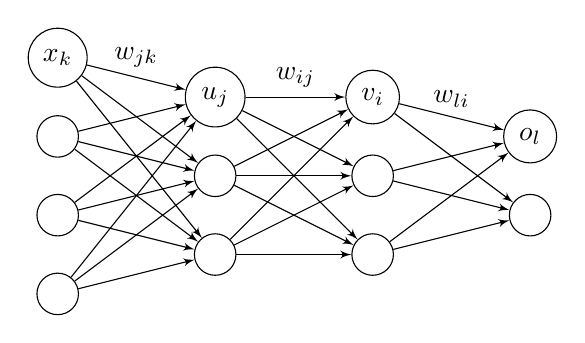
\begin{tikzpicture}

\tikzset{vertex/.style = {shape=circle,draw,minimum size=1.5em}}
\tikzset{edge/.style = {->,> = latex'}}

\node[vertex] (x1) at (0,0) {};
\node[vertex] (x2) at (0,1) {};
\node[vertex] (x3) at (0,2) {};
\node[vertex] (x4) at (0,3) {$x_k$};

\node[vertex] (v1) at (2,0.5) {};
\node[vertex] (v2) at (2,1.5) {};
\node[vertex] (v3) at (2,2.5) {$u_j$};

\node[vertex] (y1) at (4,0.5) {};
\node[vertex] (y2) at (4,1.5) {};
\node[vertex] (y3) at (4,2.5) {$v_i$};

\node[vertex] (o1) at (6,1) {};
\node[vertex] (o2) at (6,2) {$o_l$};

%edges
\draw[edge] (x1) to (v3);
\draw[edge] (x2) to (v3);
\draw[edge] (x3) to (v3);
\draw[edge] (x4) to (v3);

\draw[edge] (x1) to (v2);
\draw[edge] (x2) to (v2);
\draw[edge] (x3) to (v2);
\draw[edge] (x4) to (v2);

\draw[edge] (x1) to (v1);
\draw[edge] (x2) to (v1);
\draw[edge] (x3) to (v1);
\draw[edge] (x4) to (v1);

\draw[edge] (v1) to (y1);
\draw[edge] (v2) to (y1);
\draw[edge] (v3) to (y1);

\draw[edge] (v1) to (y2);
\draw[edge] (v2) to (y2);
\draw[edge] (v3) to (y2);

\draw[edge] (v1) to (y3);
\draw[edge] (v2) to (y3);
\draw[edge] (v3) to (y3);

\draw[edge] (y1) to (o1);
\draw[edge] (y2) to (o1);
\draw[edge] (y3) to (o1);

\draw[edge] (y1) to (o2);
\draw[edge] (y2) to (o2);
\draw[edge] (y3) to (o2);

\path[edge] (x4) -- node[above] {$w_{jk}$} (v3);
\path[edge] (v3) -- node[above] {$w_{ij}$} (y3);
\path[edge] (y3) -- node[above] {$w_{li}$} (o2);

\end{tikzpicture}

\caption{A multilayer perceptron with an input layer $x$, two hidden layers $u$ and $v$ as well as a readout layer $o$. Every connection uses a different weight $w$.}
\label{fig:mlp}
\end{figure}


A \textbf{multilayer perceptron} (MLP) is organized in several \textbf{layers}, see illustration in figure \ref{fig:mlp}. Each layer consists of a number of \textbf{neurons}.
%, the first layer has the same number as elements in the input vector $\mathbf{x}$.
Each element in the input vector $\mathbf{x}$ becomes a neuron in the input layer. Each neuron $v_i$ in the following layers gets its value by computing a weighted sum over the neurons $u_j$ in the previous layer using weights  $w_{ij}$, a bias term $b_i$ and an \textbf{activation function} $g$:

\[
v_i = g\left( b_i + \sum_j w_{ij} u_j \right)
\]

In order for the network to utilize the power of several layers, the activation function must be non-linear. If $g$ would be linear, then the entire network would be a series of linear transformations which could be rewritten as a single linear transformation. Traditional choices of $g$ include the hyperbolic tangent and the logistic function (which is sometimes referred to as the sigmoid function).

The final layer is called the \textbf{readout layer} and has as many neurons as there are classes. The input $\mathbf{x}$ is classified as the class $y$ which has the greatest value in the readout layer. In order to estimate the certainty, we can compute pseudo-probabilities $p_i$ of the classes by taking the \textbf{softmax} of the readout values $o_i$:

\[
p_i = \frac{ \exp(o_i) }{ \sum_k \exp(o_k) }
\]

\subsubsection{Backpropagation} \label{sssec:BackProp}

In order to correctly classify new input, we need to \textbf{train} the network on some existing data set $D$ which consists of pairs of correct classifications $(\mathbf{x}^{(\mu)}, y^{(\mu)}$).
We let $\mathbf{y}^{(\mu)}$ denote a \textbf{onehot} vector, that is all elements are zero except the indicated class whose associated element has the value one.
We then introduce a loss function $L$ to measure how different one network prediction $\mathbf{p}^{(\mu)}={\ldots, p_i^{(\mu)}, \ldots}$ is from its correct classification $\mathbf{y}^{(\mu)}$. Here we suggest the \textbf{squared error} loss function:

\[
L(\mu) = \frac{1}{2} \Vert
  \mathbf{y}^{(\mu)} - \mathbf{p}^{(\mu)}
\Vert ^2
\]

Given our loss function $L$, we can create a \textbf{cost} $H$ that represents the mean error over the data set $D$:

\[
H = \frac{1}{\vert D \vert} \sum_{\mu \in D} L(\mu)
\]

When $H$ is minimized, the network associates each input $\mathbf{x}^{(\mu)} \in D$ with the correct class. Since $H$ is differentiable, we can use standard \textbf{gradient descent} to optimize the network parameters, that is all weights $w_{ij}$ and biases $b_i$.
In iteration $k$ we use some \textbf{learning rate} $\eta$ and the gradient of the error $H$ to update the parameters $\mathbf{\theta}$:

\[
\mathbf{\theta}_{k+1} \leftarrow
\mathbf{\theta}_k - \eta \nabla_{\mathbf{\theta}} H
\]

\subsubsection{Stochastic gradient descent}

Since gradient descent is susceptible to local minima, it is common to use other optimization techniques such as \textbf{stochastic gradient descent} (SGD).
In gradient descent above, we let $H$ sum over all data points in $D$ in every iteration. In contrast, SGD draws a new random subset $B \subset D$ in each iteration. We refer to $B$ as a \textbf{mini-batch}. We then compute the cost $H$ as a sum over $B$ and use its gradient to update the network parameters:

\[
H = \frac{1}{\vert B \vert} \sum_{\mu \in B} L(\mu)
\]

\[
\mathbf{\theta}_{k+1} \leftarrow
\mathbf{\theta}_k - \eta \nabla_{\mathbf{\theta}} H(k)
\]

It is common to randomly partition $D$ into mini-batches so that all mini-batches are disjoint. Iterating over the entire dataset is then referred to as an \textbf{epoch}.
The random partition of $D$ should be different for each new epoch.
To achieve the wanted accuracy, it is often necessary to train over many epochs.


\subsubsection{Testing and evaluating}

Because neural networks have many parameters, they risk memorizing the training data and hence fail to learn the general patterns that we actually want them to recognize.
% \cite{AlexNet, FornesCnnCategorization}.
This phenomenon is knows as \textbf{overfitting} and can constitute a large problem for small datasets. In order to estimate overfitting, we divide the original dataset into one part for training and one for testing. The training data is used for backpropagation while the test data is exclusively used for testing. If the network begins to overfit on the training data, the accuracy on the test data decreases and the training should be aborted.

It is also common to have a third data set for evaluation which is disjoint with both the training data and the test data.


\subsection{Deep neural networks}
% Very powerful, see for example AlphaGo
% Many parameters, needs lot of data

One of the reasons why neural networks have recently achieved state-of-the-art in so many tasks is the use of very deep networks, that is networks with many layers.
% TODO add citation
The more layers, the more complex tasks can be learned. To the surprise of many, computers recently even outperformed humans in the complex game of Go \cite{AlphaGo, AlphaGoTuringTest}.

The large number of parameters in deep networks is both a strength and a weakness since it requires a large amount of training data as well as considerable computation power. More parameters can also memorize more and thus make the network more prone to overfitting \cite{AlexNet}.

\subsubsection{Dropout}

One way to reduce the risk of overfitting is by applying \textbf{dropout}  \cite{AlexNet, FornesCnnCategorization}.
%Another problem with large networks is overfitting which means that the network learns the training set by heart instead of learning to recognize the general patterns \cite{AlexNet, FornesCnnCategorization}.
The dropout method introduces a probability of setting each neuron's activation to $0$ during training, often with $50\%$ probability. This forces the network to learn multiple paths for recognizing different features and hence creating a more robust representation. Dropout also reduces the computational cost because fewer neurons participate in each training step.
Note that dropout is not necessarily done for every layer in the network.


\subsubsection{Weight decay}

Another common technique to avoid overfitting is \textbf{weight decay} \cite[Chapter~3]{NielsenBook} \cite[Chapter~7]{GoodfellowBook}. We add a new penalty term for weight regularization to our previous cost $H$, where $\mathbf{w}$ denotes all weight parameters $w_{ij}$ but not the bias parameters $b_i$:

\[
\tilde{H} = H + \alpha \Omega(\mathbf{w})
\]

The amount of regularization is determined by the hyper-parameter $\alpha \in [0,\infty)$.
A common version of weight decay is \textbf{L2 regularization}:

\[
\Omega(\mathbf{w}) = \frac{1}{2} \mathbf{w}^T \mathbf{w}
\]

By computing the gradient for the new cost metric $\tilde{H}$, we get the new update rule for the weights:

\[
\mathbf{w}_{k+1} \leftarrow
(1 - \eta \alpha) \mathbf{w}_k - \eta \nabla_{\mathbf{\theta}} H(k)
\]

We see that $\mathbf{w}$ decays with a factor $(1 - \eta \alpha)$ in each iteration, so the weights decay exponentially over time. Thus the weight decay makes sure that the weights are kept small no matter for how long the network is trained, that is no weight parameter can grow indefinitely. Empirically, it has been observed that networks can be trained longer without overfitting when the weights are bounded \cite[Chapter~3]{NielsenBook}.

Since the penalty term does not include the bias terms, the update rule for the bias parameters is unchanged.


\subsubsection{Cross-entropy loss} \label{sssec:CrossEntropy}

Above in section \ref{sssec:BackProp}, we used squared error as the loss function $L$. One of the problems with squared error is that a large error does not always result in a large gradient \cite[Chapter~3]{NielsenBook}.
A more commonly used loss function is \textbf{cross-entropy}, which has the property that its gradient depends directly on the distance between the network output and the correct value.
Thus in most cases, cross-entropy is a better choice as loss function than squared error.

For training example $\mu \in D$, we denote the network output in neuron $i$ as $p_i^(\mu)$, while $y_i^(\mu)$ takes the value one if $i$ is the correct class and the value zero otherwise. Then we can define the cross-entropy loss $L$ as:

\[
L(\mu) = - \sum_i \left(
  y_i^(\mu) \log p_i^(\mu) + (1 - y_i(^\mu)) \log (1 - p_i^(\mu))
\right)
\]

This expression may not intuitively make sense as a loss function but we can make the following observations:

\begin{itemize}
    \item Because $p_i \in (0, 1)$, both $\log p_i$ and $\log (1 - p_i)$ must be negative and thus each term in the sum is negative. We have a minus sign before the sum, so $L(\mu)$ must be positive.
    \item The correct label $y_i$ can only take the value $0$ or $1$. If $y_i=1$, then the expression can be simplified as $\log p_i$ which is greater the farther $p_i$ is from the desired value $1$. By symmetry, the same holds for when $y_i = 0$.
\end{itemize}

In conclusion we can observe that $L(\mu) \geq 0$ and is minimized when the $y_i$ predict the correct label. Furthermore, the amplitude of the loss depends directly on how far away the actual output $p_i$ is from the expected output $y_i$. Therefore, cross-entropy has the properties of a good loss function.

\subsubsection{Momentum}

One problem with stochastic gradient descent (SGD) is that the learning can zig-zag across valleys in the optimization plane, especially for noisy gradients \cite[Chapter~8]{GoodfellowBook}. Another problem is that the learning becomes very slow for stable but small gradients. A suggested solutions to both problems is the use of \textbf{momentum}. When training with momentum, instead of directly updating the parameters $\mathbf{\theta}$, we apply the gradients to a decaying momentum $\mathbf{v}$:

\[
\mathbf{v} \leftarrow \alpha \mathbf{v} - \eta \nabla_{\mathbf{\theta}} H
\]

The accumulated momentum is then applied to update the parameters:

\[
\mathbf{\theta} \leftarrow \mathbf{\theta} + \mathbf{v}
\]

With momentum, the learning no longer zig-zags across valleys because the accumulated momentum would point directly in the direction of the valley. For stable but small gradients, the learning would accelerate because the accumulated momentum grows in the same direction. Thus both problems presented above are mitigated by momentum.

\subsubsection{Alternative learning algorithms}

Although SGD is a very common technique to minimize the cost $H$, there are several popular alternatives. In stochastic gradient descent, the learning rate is a fixed hyper-parameter $\eta$ that is set manually by the programmer and is often adjusted after considerable empirical experimentation. A too high learning rate may overshoot the optimal values and hinder convergence while a too small learning rate may unnecessarily cause a long training time.

For many tasks it is desirable that the learning rate is high in the beginning when the network is very wrong while the learning rate should be small at the end when the distance to the optimal solution is small. There are several popular methods that use an adaptive learning rate: \textbf{AdaGrad}, \textbf{RMSProp} and \textbf{Adam} \cite[Chapter~8]{GoodfellowBook}. However, there is no clear consensus about which method is the best. People seem to prefer the method they are used to since their personal experience helps with setting the hyper-parameters.

Although gradient-based methods dominate the field, it is not the only possible approach. \textbf{Particle swarm optimization} has also been suggested for training neural networks in cases when it may be difficult to compute the gradient \cite[Chapter~5]{StochasticOpt}.

\subsubsection{Rectified linear activation}

Very deep networks suffer from the \textbf{vanishing gradient} problem.
Backpropagation updates each parameter according to its gradient but if the gradient is very small, it will take a long time before the network converges.
Such small gradients can occur when using the traditional activation functions, hyperbolic tangent and the logistic function, because they have very small gradients for large activations \cite{AlexNet}.
This can largely be solved by using the \textbf{rectified linear} (ReLU) function for activation: $g(x) = \max \{0, x\}$.


\subsubsection{Pre-training and transfer learning}

When the intended task has limited training data or takes a long time to train, it can be useful to start with a network that has already been trained on a different task or data set.
For example, \cite{SpatialTransformerNetworks} use the Inception network pre-trained on ImageNet.
The idea is that the parameters in a network trained on a related task is probably closer to their optimal value than randomly initialized parameters. For example, recognizing edges and corners are central to many visual recognition tasks.

% TODO: is this accurate? Book also mentions greedy pre-training such as training some layers at a time?

\subsection{Deep learning in computer vision}

Both machine translation and image captioning used to be solved by solving each subproblem separately but this kind of approach has been outperformed by end-to-end systems using deep learning \cite{ShowAndTell}. One neural network \textbf{encoded} the input to a fixed-length vector representation which was \textbf{decoded} by another network. In the case of machine translation both the encoder and decoder was implemented by an RNN which are highly suitable for processing sequences like sentences. The image captioning system was implemented in a similar manner but using a \textbf{convolutional neural network} (CNN) as encoder.


\subsection{Convolutional neural networks}

Since the publication of the AlexNet in 2012 \cite{AlexNet}, CNNs have gained large attention in computer vision for achieving state-of-the-art in various tasks such as object-detection, segmentation, video classification and object tracking \cite{InceptionV3}.

\begin{figure}
\centering

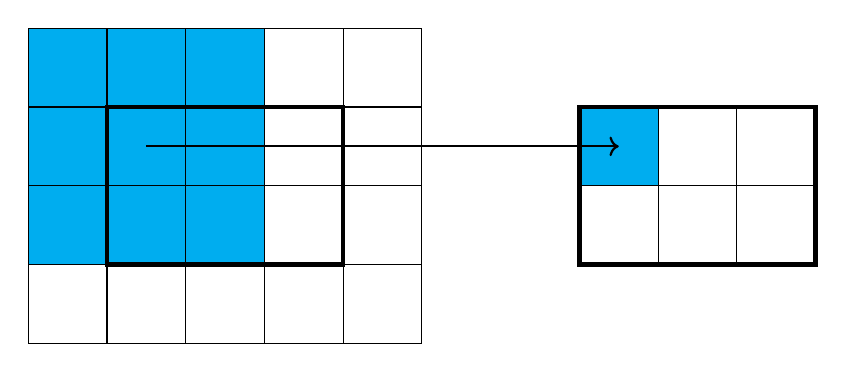
\begin{tikzpicture}
%  , fill=black!20!white
\draw [draw=black, fill=cyan] (0,1) rectangle (3,4);
\draw [draw=black, ultra thick] (1,1) rectangle (4,3);
\draw [draw=black] (0,0) grid  (5,4);

\draw [draw=black, fill=cyan] (7,2) rectangle (8,3);
\draw [draw=black, ultra thick] (7,1) rectangle (10,3);
\draw [draw=black] (7,1) grid  (10,3);

% ,very thick
\draw [->,thick] (1.5, 2.5) -- (7.5, 2.5) ;

\end{tikzpicture}

\caption{Applying a $3 \times 3$ filter to a layer of size $4 \times 5 \times D$. Note how the $3 \times 3 \times D$ region is reduced to a single scalar and how the width and depth are decreased after the operation.}
\label{fig:filter}
\end{figure}


% TODO add citations

In CNNs, each layer has a width, height and depth. Like in MLPs, the input layer has the width and height of the input image while the depth correspond to the number of color channels (one for gray scale, three for RGB and four for RGBA). We now refer to each number in the network as a \textbf{unit} instead of a neuron.

As indicated by the name, CNNs mainly consist of \textbf{convolutional layers}. The depth of a convolutional layer is determined by how many filters it has. Each filter produces a two-dimensional \textbf{activation map}, see figure \ref{fig:filter}. Each unit in the activation map comes from a weighted sum over a three-dimensional region in the previous layer over its full depth. For example a $3 \times 3$ filter applied to a 32 depth layer has $3 \cdot 3 \cdot 32=288$ weights and one bias term.
Like with MLP, the sum is passed to to a non-linear activation function such as $\tanh$. The $3 \times 3$ regions for each unit are overlapping.
The activation maps for all filters are stacked together to form a three-dimensional output, which is passed to the next layer.

Because a filter uses the same weights for all sub-regions in the previous layer, the total number of parameters are dramatically reduced compared with a fully connected layer as in an MLP. Moreover, because the same filter is applied to each sub-region, it does not matter where in the input image the object is located.

Units in higher layers in the CNN receive information from a larger \textbf{receptive field} in the input image.
% Each $2 \times 2$ pooling layer doubles the receptive field in each dimension, while every $3 \times 3$ convolutional layer increases the receptive field with 2.
Therefore, the filters in lower layers typically learn to detect low-level features like edges and curves while filters in higher layers can detect more complex objects like cats or faces.
By synthesizing the input image to maximize a specific filter's activation, it is possible to get an idea of what the filter has learned to recognize \cite{VisualizeCnn}.

\begin{figure}
\centering
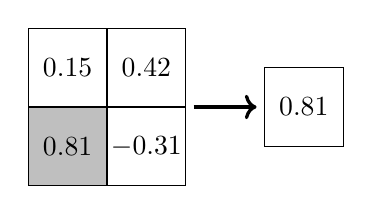
\begin{tikzpicture}

\fill[draw=black,color=lightgray] (0,0) rectangle (1,1);
\draw (0,0) rectangle (1,1) node[pos=0.5] {$0.81$};
\draw (0,1) rectangle (1,2) node[pos=0.5] {$0.15$};
\draw (1,0) rectangle (2,1) node[pos=0.5] {$-0.31$};
\draw (1,1) rectangle (2,2) node[pos=0.5] {$0.42$};

\draw (3,0.5) rectangle (4,1.5) node[pos=0.5] {$0.81$};
\draw [->,very thick] (2.1,1) -- (2.9,1) ;

\end{tikzpicture}

\caption{Example of a $2 \times 2$ max pool operation. In a $2 \times 2$ region, the largest value is chosen while the other values are ignored.}
\label{fig:maxpool}
\end{figure}


Besides filters, CNNs also use \textbf{pooling layers} in order to increase the receptive field without increasing the number of parameters in the model.
Separately for each activation map, pooling aggregates a two-dimensional region of units (e.g. $2 \times 2$) into a single unit, typically by taking the maximum value; see figure \ref{fig:maxpool}. These regions are non-overlapping so a $2 \times 2$ pooling layer decreases the representational size by 4. Thus another benefit of pooling layers is reduced computation time.

We can calculate the size of the receptive field for each output unit by doubling the field for each $2 \times 2$ pooling layer and adding $n-1$ for each $n \times n$ convolutional layer.
If we have a network that consists of two $5 \times 5$ convolutional layers with a single $2 \times 2$ maxpool layer in between, then we can compute the pixel size $r \times r$ of the receptive field as follows:

\[
r = 4 + 2(4 + 1) = 14
\]

At the end of the network, there are often a few fully connected layers (MLP) where the last layer represent the output of the network, for example pseudo-probabilities for different categories using softmax like discussed previously.

\subsubsection{Network architecture for faster computation}

The performance of CNNs typically increases with greater width and depth but it comes at a higher computational cost \cite{InceptionV3}. However, by choosing a good network architecture the same performance can be achieved but at a substantially lower computational cost, for example by refactoring large filters ($5 \times 5$, 7x7) into consecutive small filters ($3 \times 3$) and extensive use of pooling layers to reduce dimensionality. The authors also suggest a balance between depth and width of the network.

\subsubsection{Zero padding}

Applying a $3 \times 3$ filter to an input image of size 10x10 will output an image of size 8x8 since there are only 8 positions in a single row where the filter can fit. For deep networks, this shrinking might cause the final representation to become too narrow.
One can pad each activation map with zeroes to instead maintain the same size.

\subsection{Attention models}
\label{ssec:attention}
% Since waypointing only needs high-level information in a limited domain, complete transcription is unnecessary. Instead we can use recent advances in image classification.

% TODO write this part again in more detail, especially after spending more time with the literature here.

In contrast to CNNs, the human eye doesn't process the entire scene with equal precision but focuses on the most relevant parts \cite{DeepMindAttention}.
Similarly, we can let the system pay \textbf{attention} to a small part of the image at a time and successively increase the system's understanding of the image.
By choosing good locations for our attention, the important parts of the image are captured while ignoring irrelevant parts.
This reduces the computation time for training and also increases the precision of the network.
% The process of how to select a location to focus on is called an \textbf{attention model} and is often implemented using a \textbf{recurrent neural network} (RNN).
Besides image classification, attention models have also been highly successful for image captioning \cite{AttendAndTell} and machine translation \cite{machine_translation_attention}.

\subsubsection{Details}
We now describe how the attention model in \cite{AttendAndTell} works in more detail.
The goal of the attention model is to produce a vector $\mathbf{z} \in \mathbb{R}^D$ that represents the entire input image by weighing different parts of the output from the encoder CNN.

The encoder output is three-dimensional but can be seen as a grid of $L$ feature vectors. Each feature vector $\mathbf{a_i} \in \mathbb{R}^D$ corresponds to a specific location in the input image. We feed each $\mathbf{a_i}$ to an MLP which produces a scalar $e_i \in \mathbb{R}$. In the paper, the decoder uses an RNN whose hidden state is also used as input to the MLP besides the feature vector $\mathbf{a_i}$.
The scalar attention weight $\alpha_i$ for each location can then be computed by taking the softmax of $e_i$ over all units:

\[
\alpha_i = \frac{ \exp(e_i) }{ \sum_{k=1}^L \exp(e_i) }
\]

\paragraph{Soft attention}
By definition, the attention weights sum to one. A \textbf{soft attention} model computes the representative vector $\mathbf{z}$ by summing over the feature vectors $\mathbf{a_i}$, using attention as weights:

\[
\mathbf{z} = \sum_{k=1}^L \alpha_i \mathbf{a_i}
\]

\paragraph{Hard attention}
In contrast, a \textbf{hard attention} model interprets the ${\alpha_i}$ as a probability distribution over locations $i$. By sampling this distribution, $\mathbf{z}$ is chosen to be the sampled unit $\mathbf{a_i}$, ignoring the rest of the image.


\subsection{CNNs in multi-digit recognition}

Digit recognition has been studied extensively, especially for recognition of zip-codes in the US postal service \cite{lecun_1989, lecun_1990}. Originally, the digits were segmented manually and linearly transformed to a fix input size of 16x16 pixels.
Each digit image was then classified using a CNN with 3 or 4 hidden layers, with $2 \times 2$ pooling between each convolutional layer.

A complete zip-code recognition system locates the place of the zip-code and segments the zip-code into digit images \cite{zipcode_system}. The segmentation is performed by finding \textbf{connected components} (CC) in the image. If the CC has a high confidence in classification it is removed, otherwise it is either split or combined with adjacent CCs until a segmentation has been found where each classification has a high enough confidence. This is done by building a directed acyclic graph where each proposed segment is a node. The length of a path is defined as the product of the classification confidence for each node in the path. The best segmentation is then the path of greatest length in the graph. In order to avoid redundant computations, the segmentation can be done indirectly after the convolutional layers instead of on the input image \cite{lecun_multidigit}.

More recently, deep neural networks have achieved state-of-the-art in multi-digit recognition in street view images \cite{multidigit_streetview}. Instead of handling localization, segmentation and classification as separate tasks, they solve all of them using a single CNN with 11 layers. The output is modeled as a sequence $S$ of digits with a maximum length $N$. The sequence $S$ consists of a random variable $L=n$ for the length of the sequence and $n$ variables $S_i$, one for each digit. In order to handle images without numbers $L$ is allowed to have the value zero and in order to handle longer sequences than $N$, $L$ has a special value "greater than $N$". For an input image $X$, the system can be trained by maximizing $\log P(S \vert X)$. Classification is similarly done by $\text{argmax}_S P(S \vert X)$.
Because each variable has a very small domain, they can be implemented with independent softmax outputs.
Although this model works well for digit recognition of short sequences $N \leq 5$ as well as OCR in CAPTCHAs, the authors speculate that the method is not suitable for long or unbounded sequences.

Another suggested approach to digit recognition in street view is to combine CNNs with HMMs \cite{multidigit_streetview_CNN_HMM}. They use a sliding window to extract multiple overlapping frames on the input image, classify each frame using a CNN to either a digit or null and then feed the sequence of frame labels to an HMM.



\subsection{Additional topics}

Here we list some additional recent progress in the field of neural networks in computer vision which is not used in the thesis.

\subsubsection{Confidence thresholding}

Certain tasks, like automatic house number transcriptions in Google Street View, require the model to have a very high accuracy to be useful \cite{multidigit_streetview}.
For these instances, the model should output a \textbf{confidence} for its classification. If the confidence is higher than some pre-determined threshold $\tau$, we keep the prediction; otherwise we ignore the prediction and conclude that the model is not sure about that example.
% In order to increase the accuracy, the predictions that have a confidence lower than some threshold $\tau$ may be discarded.
We then need to use two metrics for evaluating the model's performance: \textbf{precision} and \textbf{recall}.

The precision measures the quality of the predictions that were higher than the threshold. It is the accuracy, or percentage of correct predictions, among the predictions that were not discarded.
% Out of the non-discarded predictions, the precision is the percentage of correct predictions.

Recall on the other hand measures how many correct predictions were discarded due to low confidence. Instead of measuring recall, we can use \textbf{coverage}, which is simply the percentage of predictions whose confidence was above the threshold $\tau$.
% TODO: is it really?
% More precisely, recall is the number of correct predictions that were not discarded divided by the total number of correct predictions.

In order to compare models, we can then plot precision vs recall or coverage for different values of $\tau$. For $\tau=0$, the precision is the same as accuracy and the coverage is $100\%$. For $\tau=1.0$, everything is discarded so the precision is $100\%$ but the coverage is $0\%$.

\subsubsection{Batch normalization}

An alternative to Dropout was suggested by \cite{BatchNormalization}. Besides reducing the risk for overfitting, the authors also suggest that it allows for a higher learning rate in deep networks and thus faster convergence.

For some network layer $\mathbf{x} = {x_1, \ldots, x_d}$, we normalize each $x_i$ to zero mean and unit variance over the current mini-batch:

\[
\hat{x_i} = \frac{x_i - E[x_i]}{ \sqrt{\text{Var} [x_i]} }
\]

We then use two learned parameters $\gamma$ and $\beta$ to instead output $z_i$:

\[
z_i = \gamma \hat{x_i} + \beta
\]

The batch normalization can thus be summarized as $\mathbf{z} = f_{BN}(\mathbf{x}; \gamma, \beta)$.

The batch normalization can either be applied before or after the activation function. The authors suggest that the best result is achieved by applying the batch normalization before the non-liner activation $g$ but after the weights $w_{ij}$ and bias $b_i$:

\[
v_i = g\left( f_{BN}\left( b_i + \sum_j w_{ij} u_j; \gamma, \beta \right) \right)
\]

\subsubsection{Visual-semantic alignment}

% Another way to model regions in the input is by using a R-CNN which have also been very successful at image captioning

Another successful approach to image captioning uses a \textbf{region convolutional neural network} (R-CNN) as encoder \cite{VisualSemanticAlignment}.
The original R-CNN method works by proposing 2000 regions in the image that are the most likely to contain an object \cite{RCNN}. Each region is then fed to a regular CNN for encoding before classification.

Since many regions overlap, it is unnecessary to compute the convolutions for them independently \cite{FastRCNN}. Instead the entire input image is processed through the CNN once and the feature vector of each region is extracted from the resulting activation map. After this improvement, the bottleneck is selecting the regions \cite{FasterRCNN}. By making a neural network to select regions from the activation map instead of from the image, the computation speed can be significantly reduced. However, this requires the training data to contain bounding boxes for the objects to detect.

In the case of image captioning, the correspondences between words and regions in the image is unknown so this relationship is modeled by latent variables \cite{VisualSemanticAlignment}.

\subsubsection{Spatial pyramid pooling}

Convolutional layers and pooling layers can handle input images of changing sizes since the filters just slide over the entire image, so the size of the output matches the input.
However, because the last layers are fully connected, they can only handle input of a fixed size. A common solution to this is to rescale or crop the input \cite{FornesCnnCategorization}. If the input consists of segmented images of handwritten words then cropping will cut away critical information while rescaling risk distorting the handwriting beyond recognition. A proposed solution to this is using a layer of \textbf{spatial pyramid pooling} (SPP).
% TODO describe SPP in more detail if relevant

\subsubsection{Spatial transformer networks}

% TODO describe Spatial transformer networks and what they are good for.
% \cite{SpatialTransformerNetworks}

\subsubsection{Residual networks}

% TODO cite Microsoft ResNet for architecture of Residual modules. There are also residual networks of residual networks.

\section{Method}

\subsection{Network architecture}


\begin{figure}
\centering

\begin{tikzpicture}
% 900, 1500, 1
% 28, 44, 256
% 1, 1, 256

%   \pic {annotated cuboid};
  \pic [fill=cyan, draw=blue] at (0,0) {annotated cuboid={width=32, height=900, depth=1500}};
  \pic [fill=cyan, draw=blue] at (2,0) {annotated cuboid={width=256, height=28, depth=44}};
  \pic [fill=cyan, draw=blue] at (4,0) {annotated cuboid={width=256, height=1, depth=1}};
  \pic [fill=cyan, draw=blue] at (6,0) {annotated cuboid={width=1, height=1000, depth=1}};

  \draw [->,very thick] (0,1) -- (2,1) {Encode};
  % ...

%   \pic [fill=magenta, text=blue, draw=blue] at (5,0) {annotated cuboid={width=2, height=50, depth=30}};
%   \pic [fill=green, text=green!50!black, draw=green!25!black] at (5,-2) {annotated cuboid={width=6, height=20, depth=15, units=mm}};
%   \pic at (1,-3) {annotated cuboid={width=150, height=200, depth=250, scale=.01, units=m}};
%   \pic [fill=cyan, text=blue!75!cyan, draw=blue!75!cyan] at (-3,-2) {annotated cuboid={width=15, height=18, depth=13.5, units=}};
\end{tikzpicture}

\caption{System overview}
\label{fig:sys_overview}
\end{figure}


We now describe the different parts of the proposed network. See figure \ref{fig:sys_overview} for an overview of how the different parts of the network interact.

\subsubsection{Encoder}

\input{figures/encoder.tex}

For encoder, we use a CNN with 7 convolutional layers with additional pooling layers, see figure \ref{fig:encoder}.
% We experimented with several different variations in number of convolution layers, pooling layers and layer depths before choosing this model.
Two consecutive 3x3 convolutional layers is a refactoring of a single 5x5 layer as suggested by \textcite{InceptionV3}. Thus, the first four convolutional layers correspond to two 5x5 convolutional layers with pooling, similar to the original single-digit CNN classifier \cite{lecun_1989} but with greater depth.

The number of pooling layers, number of convolutional layers and depth per layer were determined experimentally. The final encoder design, depicted in figure \ref{fig:encoder}, is somewhat similar to the encoder used in \cite{FornesCnnCategorization} except that we use more aggressive pooling. This is necessary because in our work, we input images of entire pages, while \textcite{FornesCnnCategorization} classify word images, which presumably are much smaller.

%The first four layers correspond closely to the original single digit classifier CNN \cite{lecun_1989} with the exception

% The number of layers and their depth was determined experimentally on the synthesized dataset using previous work as starting point \cite{FornesCnnCategorization}.



\subsubsection{Attention model}

Another major difference between our work and \cite{FornesCnnCategorization} is that although we both use variable input size, they use \textbf{Spatial pyramid pooling}, while we apply a soft attention model as presented in \cite{AttendAndTell}. As presented in section \ref{ssec:attention}, the encoder output can be seen as a list of feature vectors $\mathbf{a_i} \in \mathbb{R}^D$, which correspond to different, but overlapping, locations in the input image. The number of produced feature vectors depends on the size of the input image. We will see that this attention model aggregates all feature vectors $\mathbf{a_i}$ into a single fixed size vector $\mathbf{z} \in \mathbb{R}^D$.

The attention model consists of a multilayer perceptron, which for each feature vector $\mathbf{a_i}$ computes a salience score $e_i$:

\[
e_i = f_\text{MLP}(\mathbf{a_i})
\]

Note that this MLP does not have access to any information about the corresponding location of $\mathbf{a_i}$, thus the network must learn to recognize important parts by looking at the encoded features alone instead of learning to always look at a certain position in the input image. This is especially important for population records, where the relevant information can be in different locations depending on scribe and time period.

% We normalize the $e_i$ into $\alpha_i$ by computing the softmax.
% We normalize the $e_i$ by softmax and call the corresponding values attentions

We denote the softmax of $e_i$ as attentions $\alpha_i$, which sums to one by definition of softmax.
%We compute the softmax of $e_i$ as $\alpha_i$, which sums to one per definition.
We then use the attentions $\alpha_i$ as weights over the feature vectors:

\[
\mathbf{z} = \sum_{k=1}^L \alpha_i \mathbf{a_i}
\]

% Note that the spatial information about where in the image $\mathbf{z}$ comes from is lost in this sum.

%So just like the attention MLP, the decoder also becomes invariant to the object's position in the input image.

\subsubsection{Decoder}

The decoder employs an MLP for classifying the aggregated feature vector $\mathbf{z} \in \mathbb{R}^D$ from the attention model.
If $\mathbf{z}$ had a variable length, then we would need a different number of weights in the MLP for each different input size. Since the attention model produces a fixed size output independent of input size we avoid the problem of variable number of parameters.

Because $\mathbf{z}$ is summed over all locations, it does not contain any spatial information about where detected features come from.
Thus, the decoder is invariant to the location of detected objects, just like the attention model.

The proposed decoder MLP consists of an input layer of size $D$, one fully connected layer of $1024$ neurons with dropout and three parallel readout layers $D_1$, $D_2$ and $D_3$. Each of these three readout layers has a size of $10$ neurons and corresponds to a single digit in the range zero to nine.
Because the years we will extract are all in the range 1627--1890, $3$ digits is more than enough to classify year.

We do softmax on each readout layer to get pseudo-probabilities for the digits.
To compute the probability for a specific 3-digit sequence $\langle x, y, z \rangle$ we simply multiply the probability of each digit:

\[
P(D_1=x, D_2=y, D_3=z) = P(D_1=x) P(D_2=y) P(D_3=z)
\]


\subsection{Training procedure}
% TODO Perhaps make this a different section?

Here we describe how we train and evaluate the different models.

\subsubsection{Multi-year labels}

As presented in section \ref{sssec:swe_multiyear}, many images contain records from multiple years. However, in order to simplify the implementation, we would like all image labels to have the same size.
One way to achieve this is to simply select one of the multiple years in an image and ignore the presence of other years. However, a single year does not accurately represent images that contain multiple years.

Instead, we label each image with a tuple of the smallest and the largest year present in the image. This representation has the benefit of having a fixed size independently of how many years are in the image. Furthermore, the entire sequence of years is represented. The only information that is lost is the occasional gap in year sequences. Such gaps are often very small and also quite rare in the Swedish dataset so we assume ignoring them has a negligible effect on training and evaluation.

% TODO find gap example, how does that image look like? Does it contain the year anyway although it is not written in the label? Exactly how rare is it?

%Although it is not optimal, we currently train the network using one year as label for each image.


\subsubsection{Loss function}

We observed previously in section \ref{sssec:CrossEntropy} that cross-entropy often outperforms squared error as a loss function for classification. Cross-entropy compares a single label against the probability distribution from the network's readout layer. In our case, we output three probability distributions, one for each digit.
For a single label per image, we then have two options.
The first option is to take the cross-entropy for each digit and then sum the losses.
The other option is to take the Cartesian product of the three distributions into a single large distribution and take the cross-entropy of the combined distribution. A comparison between these two approaches is performed in section \ref{sssec:ind_digits}.

\subsubsection{Evaluation}

We evaluate the models on the test set and evaluation set of the Swedish records. Although the models only output a single year per image, we count it as $100\%$ correct if and only if the year with maximum probability is inside the label interval. For example if the label is the inclusive interval $[1771, 1774]$ and the network outputs $1773$, we count it as correct. With this relaxed definition of correctness we calculate the accuracy over the images in the respective dataset.

% TODO median distance

% TODO precision/recall if uses confidence boundary?
% problematic for multi-years: the confidence is split between different outputs...

\subsection{Extensions}

Here we discuss additional ideas that could be used to further improve our models.

\subsubsection{Multi-year loss}

It is not trivial to make a good loss function for multi-year labels. If we sum the loss for each year in the label, the images with many years have a higher influence than images with few years. Instead we can propose to take the average loss over the years but then another problem emerges: if for example the network would correctly classify an image as $1772$ where the label is $[1771, 1774]$, we still punish the network for not finding the other years.

% TODO write about experiment regarding multiyear loss.

\subsubsection{Distance loss}

Sometimes the network makes predictions that are very far away from the correct year, for example $1774$ instead of $1666$. Although we want to get the exact year, $1663$ could be considered a much better suggestion than $1774$.

One intuitive loss for distance would be squared distance. For a single year label $y$, and a probability distribution $P(X=x)$ over the years we add a distance loss $L_D$:

\[
L_D(X, y) = \sum_{x \in \{1000, \ldots, 1999\}} (y-x)^2 P(X=x)
\]

This definition of a distance loss has the wanted property that predictions far away have a big loss while predictions close to the label only give a small loss. However, there are two major problems: (1) bias and (2) independent digits.

For $L_D$ to be unbiased, the loss over a uniform distribution $U$ should be the same for all labels $y$ in the allowed interval. However, this is not the case. We can calculate the bias for different $y$ by summing $L_D$ over the allowed range. For simplicity, we map the integral year range $\{ 1000, \ldots, 1999 \}$ to a continuous range $[0,1]$ and integrate:

\[
L_D(U, y) = \int_0^1 (x-y)^2 P(U=x) dx = \frac{1}{3} + y(1-y)
\]

Thus we see that for the above definition of $L_D$, there is a strong bias for labels close to the center of the range. Likewise, a network trained with this distance loss becomes biased to suggesting years closer to the middle of the output range.

The second problem with this distance loss is that even for a perfect network, there will be considerable predictions far away from the true label because we multiply the probability distributions for the digits independently. That is, if the network is $100\%$ certain that the last two digits should be $3, 4$ and the correct label is $1834$, we will still get strong signals for $1734$ and $1634$.

\subsubsection{Proximity score}

\textbf{TODO: delete this section about Proximity score? The idea does not really seem helpful...}

In order to solve the first problem we could suggest another approach: instead of minimizing a distance error, we can maximize a proximity score $S_D$ using a weight function $W$ around the label $y$:

\[
S_D(X, y) = \sum_i P(X=x) W(x, y)
\]

Because we want to reward predictions near $y$, we can use a truncated Gaussian as weight function:

\[
W(x, y) = \exp \left( \frac{-(y-x)^2}{\sigma^2} \right)
\]

We can then compute the bias in the same way as before, by integrating over a mapped interval $[0,1]$:

\[
S_D(U, y) = \int_0^1 P(U=x) W(x, y) dx =
\int_{-y}^{1-y} \exp \left( \frac{-x^2}{\sigma^2} \right) dx
%\frac{\sigma \sqrt{\pi}}{2} \left(
%\text{erf} \left( \frac{1-y}{\sigma} \right) +
%\text{erf} \left( \frac{y}{\sigma} \right)
%\right)
\]

We see that there is a bias for labels $y$ near the edges of the range, but for most values of $y$, the bias is negligible for small values of $\sigma$.

\subsubsection{Auxiliary input}

So far we have not utilized the information that pages in a book come in sequences, thus if the previous page was $1771$, the following page has a strong probability of either being $1771$ or $1772$. This additional information could be taken into account by letting the network have the prediction of the previous page as an auxiliary input to the decoder. However, there are some problems with this. Firstly, it is not clear what the auxiliary input should be for the first page in a book. Secondly, during training we want to draw the images in a random order to prevent overfitting. However, we can not classify the previous image again because we would be missing the auxiliary input of that image. Instead, we could use the predictions from the previous epoch. Then the predictions used for auxiliary input would have been produced by presumably rather different weights than the current version of the decoder employ. We hypothesize that this temporal mismatch between decoder weights would introduce randomness and make learning from the auxiliary input slow and/or unstable.

\subsubsection{Post-processing}

Another approach to use the sequential information of books is to post-process the predictions. For example, if the network would suggest the sequence $\langle 1771, 1872, 1773 \rangle$, we could correct it to $\langle 1771, 1772, 1773 \rangle$. We suggest using the \textbf{Viterbi algorithm} on the following model to attempt to correct the predictions.

For each image $t$, we define $z_{tj}$ to be the model's prediction probability that page $t$ has label $j$. We also introduce a jump distribution $Q(j, k)$ for making a transition from label $j$ to label $k$.

With this model, we consider each book to be a sequence of state transitions. A transition at time $t$ from state $j$ to state $k$ is calculated as $z_{tk} Q(j, k)$. We can then apply the Viterbi algorithm using \textbf{Dynamic programming} to find the maximum probability sequence of state transitions.

We create a matrix $T$ that for each page $t$ contains the maximum probability of a sequence so far. For the first page, we simply take the network predictions: $T[0,j] = z_{0j}$. For every other page, we introduce the following recurrence:

\[
T[t,j] = z_{tj} \max_k \left\{ T[t-1,k] Q(k, j) \right\}
\]

After computing the entire matrix $T$, the probability of the most likely sequence is the largest value in the last column of $T$. We can then reproduce the most likely sequence by backtracking.

To make the algorithm run faster, we only allow labels in a smaller interval 1600--1899 instead of the possible output 1000--1999.

\paragraph{Creating $Q$}
The jump probability $Q(j, k)$ can be found by statistically counting the page transitions in the training data. We simplify the distribution by only taking into account the year difference between $j$ and $k$. In order to handle unseen transitions, we use \textbf{Laplace smoothing} with $\alpha=0.5$. We denote $N(r)$ as the count of year transitions with difference $r$, $N$ to be the total number of transitions and $K$ to be the number of allowed labels.

\[
Q(j, k) = Q(k-j) = \frac{N(k-j) + \alpha}{N + \alpha K}
\]

For images that have multiple years, we uniformly distribute the weight between the possible transitions of the two images. A transition from $[1771, 1772]$ to $[1772, 1773]$ would thus produce the following count: {0: 0.25, 1: 0.5, 2: 0.25}.

% TODO: mention conditioning

% For each image $t$ the network outputs a probability distribution for a three digit sequence $\mathbf{z}_t \in \mathbb{R}^1000$ so that $P(D_1=x, D_2=y, D_3=z) = z_{tj}$.

\subsection{Tensorflow}
% TODO should technologies/implementation be described in a different section?
% Is it at all relevant to discuss about Tensorflow?

% TODO Mention GPU acceleration here or in section about neural networks or Hardware?

\subsection{Hardware}
% TODO Mention hardware and training time .


% Outcome
\chapter{Results and discussion}

\textit{
In the previous chapter we described our main model and training procedure as well as some alternatives.
In this chapter we describe the numerical results of our implementation of the main model on two datasets, one synthetic dataset created from MNIST and the much more difficult Swedish population records. We also perform several experiments where we change the model configuration or training procedure and observe the effect on either or both datasets.
Hopefully, our observations can be instrumental in
% TODO: instrumental? Rephrase?
designing future encoder-decoder networks.
}

\section{Simulations on synthetic data} \label{sec:simulations}

Since the images of the Swedish records are so large, we decided to create a simpler and faster dataset so we could quickly iterate on the network architecture. Here we describe the synthetic dataset we created as well as some observations from altering the network configuration.

\subsection{Four-digit MNIST}


\begin{figure}
    \centering
    \begin{subfigure}[b]{0.45\textwidth}
        \centering
        \includegraphics[scale=2.0]{resources/mnist4.jpg}
        \caption{Four digits without noise.
        %, size $112 \times 28$.
        }
        \label{fig:mnist4}
    \end{subfigure}%
    \begin{subfigure}[b]{0.45\textwidth}
        \centering
        \includegraphics[scale=2.0]{resources/random_pad.jpg}
        \caption{Random position and dot noise.
        %Four digits with noise.
        %at a random position inside a box of $168 \times 56$ with dot noise.
        }
        \label{fig:mnist_random_pad}
    \end{subfigure}
    \caption{Two examples of generated synthetic data from MNIST.}
\end{figure}

For our early experiments we created a synthetic dataset with small images of four-digit sequences.
Each image was a concatenation of four independently randomly selected digit images from MNIST \cite{MNIST_orig}, where the first digit was always a one. See figure \ref{fig:mnist4} for an example. The resulting image was then a fixed size of $28 \times 112$ pixels.
%, compared to $900 \times 1500$ or more for the downsampled Swedish records.
% which is very much smaller than the images of the Swedish records.
Because the images were so small, it took a much shorter time to train and evaluate different models on the synthetic dataset than on the Swedish population records, whose images were very large.

Several models performed very well on this task, one of them achieving $94\%$ accuracy after 10,500 cpu-seconds of training. These models are discussed further in section \ref{sssec:exp_encoder}.

\subsection{Noisy MNIST}

In order to make the synthetic data a little bit more difficult to classify and more similar to the Swedish dataset, each four-digit image was placed at a random position in a larger image whose pixel values were zero, that is no ink.

When putting the four-digit image at a fixed position instead of a random position, one model learned to encode the distance from the left side of the image, which is quite interesting considering that neither the attention model nor the decoder had any explicit access to spatial information.
When adding $100$ additional zero-pixels to the right of the image, the accuracy dropped from $85\%$ to $80\%$. However, when adding $4$ zero-pixels to the left, the accuracy dropped to only $1\%$. We attribute this sudden accuracy loss to the difficulty of identifying which digit to keep and which to ignore. Since we are training on four-digit images but only expect the last three, the model must learn to find but ignore the first digit.
Since the year can appear at any position in the Swedish data, the simulations should also vary the position of the digits. Therefore, we must use random positions instead of fixed positions for the synthetic data.

Finally, we applied dot-noise to the image by:
(1) inverting the image so that the background is represented by one instead of zero,
(2) multiplying each pixel value with a random number drawn independently uniformly from $[0.6, 1.0]$ and
(3) inverting the image back again.
This corresponds to adding a random but small amount of ink to each pixel in the image.

An example image with dot noise and random position can be seen in figure \ref{fig:mnist_random_pad}. The models were evaluated on the image size $56 \times 168$ pixels, like in the figure.


\subsection{Network depth and width} \label{sssec:exp_encoder}

By running a time trace on the training operation, we saw that the majority of the training time was spent on applying and updating the encoder network. In order to reduce training time we performed the following experiments to design a more efficient encoder network while maintaining a good accuracy on the simulation tasks.
% TODO: insert graph?

% By counting the number of trainable parameters in the model we observed that the majority of parameters are contained by the MLPs in the attention and decoder model.

\subsubsection{Simulations on noise-free data}

Earlier in section \ref{sec:method_architecture} we presented a model architecture that we now refer to as DEP. We will come back to this model soon. In our initial experiments however we used another model for baseline, which we call DE. The DE encoder consisted of four blocks where the first three blocks contained two $3 \times 3$ convolutional layers and one $2 \times 2$ pooling layer. The last block contained a single $1 \times 5$ convolutional layer and one $1 \times 2$ pooling layer.
The main difference between DE and DEP is that DEP used one additional pooling layer between the two consecutive convolutional layers in the third block.
% The only difference between DEP and DE is that DEP had one additional pooling layer between two convolutional layers near the end of the encoder.
We will see that this small difference had a great impact on accuracy and running time.


\begin{figure}
    \centering
    \begin{subfigure}[c]{1.0\textwidth}
        \centering    \includegraphics[scale=0.5]{resources/mnist_4_graph.png}
        \caption{Four-digit MNIST without noise.}
        \label{fig:mnist_early_models}
    \end{subfigure}
    \begin{subfigure}[c]{1.0\textwidth}
        \centering
        \includegraphics[scale=0.5]{resources/model_experiments.png}
        \caption{Noisy MNIST.}
        \label{fig:mnist_models}
    \end{subfigure}
    \caption{Plot of accuracy vs training time measured in CPU seconds for several models. Each data point comes after one epoch of training.}
\end{figure}


In figure \ref{fig:mnist_early_models} we can see the resulting accuracy over training time of the different variations of the DE model.
All configurations used cartesian loss (defined in section \ref{sssec:cartesian}) and soft attention (defined in section \ref{sssec:soft_attention}).

% For baseline we use a model called DE, which is rather similar to the model presented earlier in section

% The DE model was used as baseline with an encoder that had 7 layers and an output depth of 256. It is very similar to the DEP encoder illustrated in figure \ref{fig:encoder} except that it used one less pooling layer.

The model called DED was the same DE except that the decoder depth was halved from 1024 to 512. In figure \ref{fig:mnist_early_models} we can see that doing so had little impact on the accuracy and training time.

In another experiment, which we refer to as DEL, we halved the depth of every encoder layer. Halving the depth of every encoder layer halves the representational size in the encoder and consequently halves the training time. However, simplifying the encoder like this also seems to have limited its learning capability. In fact, it had about the same accuracy per training time as the DE model.

% When halving the depth of the DE decoder from 1024 to 512, (DED) had little impact on this task.
% Halving the number of filters in every layer (DEL) halved the training time per epoch but also halved the learning rate, so in the end its performance was about the same.

% The TE model was identical to DE except that it used fewer convolutional layers. More precisely, the DE encoder started with $\langle C,C,P,C,C,P \rangle$ while TE started with $\langle C, P, C, P \rangle$, where $C$ stands for $3 \times 3$ convolution and $P$ stands for $2 \times 2$ max-pooling.

% In both the DE model and the DEP model, the encoder had two consecutive convolutional layers at two places in the beginning of the encoder. These double layers in the DEP model can be seen in figure \ref{fig:encoder}.
In order to reduce the training time, we experimented with
simplifying the DE encoder by removing the second convolutional layer in each of the first two blocks. We call this thinner model TE.
% removing two convolutional layers so that there would be no consecutive convolutional layers. So in the model we call TE, every second layer in the encoder was a max-pool layer.
Similarly to the model DEL described above, where we simplified the encoder by halving the depth of each layer, both training time and accuracy was reduced. When plotting accuracy against training time in figure \ref{fig:mnist_early_models}, we see that just like DEL, the TE model was comparable to DE.

We also tested a variant to TE where an additional pooling layer was added between the two convolutional layers in the third block. So in this new model, which we call TEP, every second layer is a pooling layer.
Compared to TE, the TEP model learned much quicker. However, TEP started to overfit after hitting $90\%$ accuracy while the baseline model DE continued to improve until $94\%$.

% When adding an additional pooling layer (TEP) to the thinner model (TE), learning increased very rapidly for the first two epochs. However, it started to overfit after hitting $90\%$ accuracy, while the accuracy of the baseline model (DE) continued to rise to $94\%$.

In summary we can see that models with smaller representational size achieves about the same accuracy given the same amount of training time, although the heavier models seem to have higher potential in the long run. Another observation is that additional pooling can greatly increase the learning rate in the beginning of training.

% The learning rate on the simpler four-digit MNIST dataset for different some possible configurations of the encoder.

% By training on the simpler four-digit MNIST dataset without noise,
%we made several observations.
% We experimented on various configurations of encoder and decoder depth and width.
% we found that increasing the width of the decoder's hidden layer from 512 to 1024 had a very small impact on the training time while increasing accuracy. Decreasing the number of layers in the encoder from 7 to 5 decreased the accuracy somewhat but increased training time considerably. Halving the encoder width halved the training time but also decreased accuracy. Adding a pooling layer at the end of the encoder resulted in a higher accuracy after the first epoch and reduced training time. The effect of an extra pooling layer can be seen by comparing the models TE and TEP in figure \ref{fig:mnist_early_models}.

\subsubsection{Simulations on noisy data}

The best configurations so far were evaluated on the more difficult synthetic dataset with random positions and noise. Figure \ref{fig:mnist_models} contains a comparison between some variations of encoder configurations on the noisy MNIST dataset.
By comparing this graph to figure \ref{fig:mnist_early_models}, we can see that using larger input images, placing the digits at a random position and adding noise makes the problem much more difficult. Training a single epoch takes almost three times as long and the increase in accuracy per epoch is reduced considerably.
%Note that for the same model, we needed to train more than 4 times longer to get the same accuracy as on the simpler synthetic dataset.

The three best configurations (DEP, DEB, DEM) achieved very similar results considering the test accuracy vs training time. These three configurations had the same number of encoder layers but different depth of each layer.

The heaviest encoder DEP is illustrated in figure \ref{fig:encoder}.
Because it had the most number of filters, the training time for each epoch was much longer than for the other two alternatives.
% For this encoder the representational size of the input decreases exponentially for each pooling layer: 32, 16, 8, 4, 2.
Since each pooling layer divides the representational size by four and the number of filters in this model doubles after almost every pooling layer, the representational size decreases is halved after most pooling layers.

While the representational size decreases for DEP, as recommended by \textcite{InceptionV3}, the DEM encoder was designed to keep the representational size as constant as possible from the start.
This was done by reducing the layer depth to a minimal amount, with only 4 filters at the input layer instead of 32.
As we can see in figure \ref{fig:mnist_models}, the training time for each epoch was much faster although the actual learning over time was almost the same as for the DEP model.

The third competing encoder DEB was a middle ground between DEP and DEM, designed to have a very slowly decreasing representational size.

\subsubsection{Wider encoders are more robust to varying input size}


\begin{figure}
    \centering
    \includegraphics[scale=0.6]{resources/mnist_resilience.png}
    \caption{Three encoder configurations were trained independently for 31,000 cpu-seconds on the noisy MNIST dataset, with an input size of $56 \times 168$. The graph shows the accuracy of the trained models on increased input size without any retraining.}
    \label{fig:mnist_resilience}
\end{figure}

When increasing the size of the generated synthetic images without retraining the models, the accuracy of the DEP model was relatively stable even for the double width and height but dropped for larger input. The two lighter models, DEB and DEM, were less robust to this change in input; see figure \ref{fig:mnist_resilience}.

The attention model is responsible for choosing the correct location in the input image. The receptive field of output units in the three configurations were the same and the architecture of the attention model was identical. The background noise was also identical. So although the attention model worked well for a smaller image, it is not sure it may work as well for a larger image where the background is the same.
% One possible reason for this is that the soft attention for all locations must sum to one. Since there are more locations to choose from, the weight on the correct location decreases.
Remember that the attention model does not know how many locations there are but outputs a salience score for each location independently. Since we use the softmax of these salience scores, the resulting attention weights must sum to one. So the more locations there are, the more the attention risk to spread out over noisy locations. To counter this, the attention model would have to be even more aggressive to separate background noise from useful signals. For hard attention however, only the most promising location is kept and the rest are ignored. So a model trained with hard attention should be more resilient to increased image size. We discuss more about attention later in section \ref{sssec:result_attention}.

We see that the more filters a model has, the more stable it is to change. Hence we believe that although on a single task the three configurations performed comparatively, the heavier model generalizes better in the long run.

% We attribute this resilience to noise to detecting more features in the input, some of which are better preserved after adding the noise.


% We argue that the heavier model, DEP, with its additional filters can detect more features in the input

% The lightest encoder (DEM) was designed to have the same representational size as DEP at the end of the encoder but decreasing the number of filters in the beginning in order
% keeping the representational size as constant as possible from the start by using fewer filters, in contrast to the advice from \textcite{InceptionV3}.


\section{Experiments on Swedish population records} \label{sec:experiments}

In this section we present and discuss our model with variations on the Swedish population records.
% metrics of different models and training
% comparisons we made between different models on the Swedish population records.

\subsection{Setup}
 Here we describe the platform on which we evaluated the models.

\subsubsection{Downsampling}
The images of the Swedish population records had a high resolution so they were downsampled with a ratio of 8. For example instead of having a size of $4688 \times 6360$ an image would have the size to $586 \times 795$. Because the images have different sizes, in each batch the images were padded with zeroes to get the same size as the largest image in the batch.

\subsubsection{Implementation}
The models were implemented in Tensorflow \cite{Tensorflow}, which is a popular open-sourced machine learning framework. The implementation\footnote{\url{https://github.com/HalfLeif/CNN_doc_extraction}} is freely available on Github.

\subsubsection{Hardware}
We trained the models on 3 threads on a single Intel(R) Core(TM) i7-4770K @ 3.50GHz. Training a single epoch of Swedish population records took about 28 hours. It would be faster to train using more threads or GPU acceleration but we were constrained by limited access to hardware.


\subsubsection{Pre-training}

All experiments in this section start with a pre-trained model already. Most of them use a model we refer to as the \textbf{base model}. The base model used the DEP encoder and was trained using soft attention and cartesian loss for 5 epochs on the noisy MNIST and then for 16 epochs on the Swedish population data. Thus it had an accumulated training time of more than 4,200,000 cpu-seconds or almost 3 weeks on our hardware.
% noisy MNIST DEP-5: 41,217 cpusec ?
% 16 epochs of SweDEP: 264775*16 cpusec = 4,236,400
% SUM:
The base model had an accuracy of $8.39\%$ on the main test set and an accuracy of $2.11\%$ on the second test set.

Optimally, the model variations should be retrained from scratch but doing so would simply take too long time.
Instead, we present the observed accuracies as a lower bound to the potential of each observation and as an indication of whether the variation was helpful or not.
% Since the models were heavily pre-trained with a different configuration, we present our observations as a lower bound to the potential accuracy of each variation.

% that pre-trained on the noisy MNIST for 5 epochs which was then trained on the Swedish population data

% The experiments in this section were performed after training the model for many epochs on the Swedish data already. Optimally we would want to retrain the model from scratch for each alteration but doing so would take too much time. Thus we can only provide a lower bound for the accuracy of the altered models.


\subsection{Independent digits vs cartesian loss} \label{sssec:ind_digits}

We now compare using the independent digit loss presented in section \ref{ssec:method_loss} against the cartesian loss introduced in section \ref{sssec:cartesian}.
% TODO: check in notes for results on MNIST data.
Training the DEP configuration from scratch on the noisy MNIST data using either loss function gave very similar results although the training time was slightly longer for cartesian loss.

For the Swedish population records, the base model used cartesian loss already. When training one additional epoch using the independent digit loss, the test accuracy dropped from $8.39\%$ to $7.2\%$. However, when training the model for another six epochs we reached the test accuracy of $8.98\%$. This model we refer to as base2 because some of the following models were trained from this model.

\subsection{Multi-year vs single-year loss} \label{ssec:result_multiyear}

Both the cartesian loss and independent digit loss discussed above only used a single year from the label. We suggested another loss function in section \ref{sssec:alt_multiyear} that takes into account the full year interval in the label by averaging the loss function over all years in the label interval. Now we compare using the multi-year vs the single-year version of independent digit loss.

As mentioned above, when changing the loss function for the base model to single-year independent digit loss for one epoch, the accuracy dropped from $8.39\%$ to $7.2\%$. However, when instead changing it to the multi-year version, the accuracy dropped even further to $7.07\%$. When training with multi-year loss from base2 for four epochs, the test accuracy dropped from $8.98\%$ to $7.58\%$

Although the test accuracy for the multi-year model decreased, the accuracy on the second test set increased from $2.35\%$ to $2.75\%$. This is the best result we have achieved on the second test set, which tests the model on completely new books from other regions.

In conclusion, the multi-year loss decreased the accuracy on the main test set but improved the model's ability to generalize to new collections.
One possible cause for this may be that multi-year loss makes the network focus more on the handwritten digits instead of the handwriting. However, when comparing the attention for the two models on the same images they look quite similar.


\subsection{Simplifying the training data}

When a page contains multiple valid years, our single-year loss function only rewards finding the highest year and penalizes all other years, including valid ones.
In our previous experiment, we attacked this problem of miss labeling in our training data by making a loss function that takes into account all the years in the label. In this experiment, we instead try to estimate the impact of miss labeling by only training on images that have a single year in it. Here we again the use single-year independent digit loss function.

After training for one additional epoch beyond the base2 model, the test accuracy dropped from $8.98\%$ to $8.83\%$.
After another five epochs, we reached the highest seen test accuracy of $9.54\%$. On the other hand, the accuracy on the second test set was an all-time low at $1.42\%$.

\subsection{Soft vs hard attention} \label{sssec:result_attention}

So far, all reported models have used soft attention. Hard attention uses the same network, the only difference is that instead of doing a weighted sum over the encoded locations, we choose one of them. In previous work, the hard attention has seen the attention weights as a distribution over the location and samples that distribution. In our work however, we simply choose the location with highest attention weight.


\begin{figure}
    \centering
    \includegraphics[scale=0.6]{resources/soft_vs_hard.png}
    \caption{The DEP model learns much faster with soft attention on the noisy MNIST dataset.}
    \label{fig:attention_mnist_graph}
\end{figure}


When training the DEP model with hard attention from scratch on the noisy MNIST data for one epoch, we only got a test accuracy of $4.4\%$ instead of $17.2\%$.
In figure \ref{fig:attention_mnist_graph} we can see how much quicker the DEP model learns to recognize digit sequences using soft attention.


\begin{figure}
    \centering
    \begin{subfigure}[c]{0.45\textwidth}
        \centering    \includegraphics[scale=2.0]{resources/MNIST_soft_att/1177_att.jpg}
        \caption{Soft attention in white on the image to the right. It correctly focused more to the bottom and left.}
        % \label{fig:mnist_early_models}
    \end{subfigure} \quad %
    \begin{subfigure}[c]{0.45\textwidth}
        \centering
        \includegraphics[scale=2.0]{resources/MNIST_soft_att/1177_correct.jpg}
        \caption{The image was correctly classified as 1177.}
        % \label{fig:mnist_models}
    \end{subfigure}
    
    \vspace{1em}
    
    \begin{subfigure}[c]{0.45\textwidth}
        \centering    \includegraphics[scale=2.0]{resources/MNIST_hard_att/1281_att.jpg}
        \caption{Hard attention in white of the image to the right. The attention only captured part of the number.}
        % \label{fig:mnist_early_models}
    \end{subfigure} \quad %
    \begin{subfigure}[c]{0.45\textwidth}
        \centering
        \includegraphics[scale=2.0]{resources/MNIST_hard_att/1281_fail_1031.jpg}
        \caption{Input image with label 1281, it was incorrectly classified as 1031.}
        % \label{fig:mnist_models}
    \end{subfigure}
    \caption{Examples of soft and hard attention applied to noisy MNIST images with sizes $312 \times 136$.}
    \label{fig:attention_mnist}
\end{figure}


In figure \ref{fig:attention_mnist} we can see how the soft attention successfully captured the year by putting together information from several locations. In the same figure, the hard attention fails because it can only see some of the digits.


\begin{figure}
    \centering
    \begin{subfigure}[c]{1.0\textwidth}
        \centering    \includegraphics[scale=0.56]{resources/SWE_attention/S3HT-64P3-T61.jpg}
        \caption{The correct year is 1813; it is emphasized in the picture with ellipses.}
    \end{subfigure}

    \vspace{1em}

    \begin{subfigure}[t]{0.45\textwidth}
        \centering
        \includegraphics[scale=1.0]{resources/SWE_attention/SoftAtt/att_S3HT-64P3-T61.jpg}
        \caption{The base model correctly classifies the image as 1813. The attention correctly focuses on the year as well as on some handwriting.}
    \end{subfigure} \quad %
    \begin{subfigure}[t]{0.45\textwidth}
        \centering    \includegraphics[scale=1.0]{resources/SWE_attention/HardAtt/att_S3HT-64P3-T61.jpg}
        \caption{The hard attention model predicts the page as 1899 because it is looking at the wrong location.}
    \end{subfigure}

    \caption{Soft vs Hard attention on an image from the main test collection. The page comes from the book Asker C:4 in the Örebro collection.}
    \label{fig:attention_dep_T61}
\end{figure}


\begin{figure}
    \centering
    \begin{subfigure}[c]{1.0\textwidth}
        \centering    \includegraphics[scale=0.29]{resources/SWE_attention/S3HY-DRC3-H5L.jpg}
        \caption{The correct year is 1814, although the year is actually not written in the page but inferred from previous pages.}
    \end{subfigure}

    \vspace{1em}

    \begin{subfigure}[t]{0.45\textwidth}
        \centering
        \includegraphics[scale=1.0]{resources/SWE_attention/SoftAtt/att_S3HY-DRC3-H5L.jpg}
        \caption{The base model classifies the image as 1811 by looking at the handwriting.}
    \end{subfigure} \quad %
    \begin{subfigure}[t]{0.45\textwidth}
        \centering    \includegraphics[scale=1.0]{resources/SWE_attention/HardAtt/att_S3HY-DRC3-H5L.jpg}
        \caption{The hard attention model predicts the page as 1760.}
    \end{subfigure}

    \caption{Soft vs Hard attention on an image from the main test collection. The page comes from the book Axberg C:5 in the Örebro collection.}
    \label{fig:attention_dep_H5L}
\end{figure}


When training the base model for one epoch with hard attention on the Swedish population records, the accuracy dropped from $8.39\%$ to $2.19\%$.
In figure \ref{fig:attention_dep_T61} we see how the soft attention partially focuses on the year and gets the prediction right while the hard attention focus on the place for the image id rather than the year.
Another example can be seen in figure \ref{fig:attention_dep_H5L} where the year is not written on the page. The soft attention guesses the correct decade by looking at the handwriting all over the page while the hard attention suggests the wrong century.

In conclusion, we see that the models with soft attention use information from all over the page to make its prediction. This includes several written years if any as well as the handwriting.
However, the single location chosen by the hard attention model does not contain enough information for making a good prediction.

Even for the simpler problem of noisy MNIST, hard attention failed because it only captured part of the digit sequence. Soft attention on the other hand could reconstruct the digit sequence by choosing multiple close locations.


\section{Post-processing} \label{sec:result_post_process}

The best result on the second dataset had an accuracy of $2.75\%$, using multi-year loss. When running the post-processing on the predictions of this model, the accuracy was increased to $3.58\%$. So even though the original predictions were quite noisy, the post-processing could still use them to boost the accuracy further.

We also tested the post-processing on the indexed part of the Örebro collection. Note that this collection was partitioned for both training and testing, so $90\%$ of the predictions are on training data. The accuracy of base2 was $14.9\%$ on this collection. Post-processing increased the accuracy to $15.9\%$. The mean distance between the prediction and the label was also reduced from 6 years to 4 years after post-processing.

% Works Örebro, Asker-C-2 189:
% 	 S3HT-64P3-KY5 1768 1768 [1768]
% 	 S3HT-64P3-PS4 1768 1768 [1768, 1769]
% 	 S3HT-64P3-KTG 1768 1768 [1769]
% 	 S3HT-64P3-T3Q 1771 1769 [1769]
% 	 S3HT-64P3-R81 1771 1770 [1769]
% 	 S3HT-64P3-V2C 1777 1771 [1769]

% Fail Asker-C-3 147:
% 	 S3HT-64P3-2W5 1798 1798 [1797]
% 	 S3HT-64P3-T75 1795 1798 [1797]
% 	 S3HT-64P3-NXY 1798 1798 [1797, 1798]
% 	 S3HT-64P3-233 1798 1798 [1798]
% 	 S3HT-64P3-KRW 1805 1808 [1798]
% 	 S3HT-64P3-RZP 1798 1808 [1798]

\begin{table}
\begin{subtable}{\linewidth}
\centering
\begin{tabular}{|c|c|l|}
    \hline
    Before & After & Correct \\
    \hline
    1768 & 1768 & 1768 \\
    1768 & 1768 & 1768, 1769 \\
    1768 & 1768 & 1769 \\
    1771 & \textbf{1769} & 1769 \\
    1771 & 1770 & 1769 \\
    1777 & 1771 & 1769 \\
    \hline
\end{tabular}
\caption{The post-processing can correct one of the pages to 1769. Although 1771 is not correct for the last page in the example, it is still closer to the true value than the prediction 1777.
The pages are an extract from the book Asker C:2.
}
\end{subtable}

\vspace{1em}

\begin{subtable}{\linewidth}
\centering
\begin{tabular}{|c|c|l|}
    \hline
    Before & After & Correct \\
    \hline
%   \textbf{h [m} & \textbf{dim [m} \\ \hline
    1798 & 1798 & 1797 \\
    1795 & 1798 & 1797 \\
    1798 & 1798 & 1797, 1798 \\
    1798 & 1798 & 1798 \\
    \textbf{1805} & 1808 & 1798 \\
    1798 & 1808 & 1798 \\
    \hline
\end{tabular}
\caption{
The network makes a confident but incorrect prediction that the century digit should be 8 and the decade digit 0. The incorrect prediction makes the post-processing prefer 1808 over the true value of 1798.
The pages are an extract from the book Asker C:3.
}
\end{subtable}
\caption{Two examples of post-processing. In the column to the left is the prediction made by the model, the middle column contains the updated prediction after post-processing and the rightmost column contains the true label.}
\label{tab:post_process_example}
\end{table}


In table \ref{tab:post_process_example} we can see some examples of the post-processing applied to books in the Örebro collection. The post-processed sequence is typically very smooth compared to the raw predictions. Sometimes a single confident but incorrect prediction can start a long sequence of errors. One of the reasons for this is that the jump distribution strongly prefers increasing the year over decreasing the year.

\subsection{Jump distribution}


\begin{figure}
    % \centering
    % \begin{subfigure}[c]{1.0\textwidth}
        \centering        \includegraphics[scale=0.7]{resources/jump_distribution.png}
        \caption{The jump probability calculated from the training set and main test set.
        As expected, the following page is most likely the same year or the consecutive year. With laplace smoothing of $0.5$, the probability for a zero-transition is $56.5\%$ and the probability for a plus-one-transition is $29.1\%$. The interval $[-1,5]$ contains $95.5\%$ of the smoothed distribution.}
        \label{fig:jump_prob}
    % \end{subfigure}
    % \begin{subfigure}[c]{1.0\textwidth}
    %     \centering
    %     \includegraphics[scale=0.7]{resources/jump_log_counts.png}
    %     \caption{The plot shows $\log(1+\text{count}(x))$ for each label transition $x$.}
    %     \label{fig:jump_log_counts}
    % \end{subfigure}
    % \caption{The jump probability calculated from the training set and main test set.}
\end{figure}


The major chunk of the jump probability distribution is illustrated in figure \ref{fig:jump_prob}. We see that most page transitions should either keep the same year or increase by one.
As described earlier in section \ref{sssec:alt_postproc}, when counting transitions between two pages where both pages have multiple years, we give fractions of count to all combinations of years. This results in the small probabilities for minus one and plus two et cetera, which can be seen in the probability distribution.
% Because of multi-year labels, we also have small probabilities for minus one and plus two, since we count all combinations of .

It also happens in some books that there is a major leap between two pages as a new section of the book begins. This can be seen in the log counts for the four main collections of the Swedish population records, which is plotted in figure \ref{fig:jump_log_counts}.

\subsection{Conditional jump distribution}
One problem with the above jump distribution is that, for our dataset, a vast majority of the page transitions are zero jumps; that is from the same label to itself.
Because the distribution heavily favors the zero jump, the predictions after post-processing often output the same year for all pages in a book, instead of increasing years as we would expect.

One idea to fix this is to condition the current transition on the previous transition. The idea is that if the previous transition was a zero jump, we should be more likely to change year now. However, when aggregating the statistics for the Swedish dataset, it turns out our intuition was wrong: if the previous transition was a zero jump, it is even greater probability that the current transition is a zero jump. So a conditional distribution reinforces the problem instead of alleviating it.


\section{Model comparison}

%  & Swe_DEP_7-199 & 0.0417 & 10 & 18 & 0.262 &  &  &  &

\begin{table}
  \centering
  \begin{tabular}{|c|c||c|c|c|c||c|c|c|c|}
    \hline
    Name & Epochs & Acc & Med & Mean & Near & Acc & Med & Mean & Near \\
    \hline
    Base & 16 & 0.0839 & 6 & 10 & 0.408 & 0.0211 & 23 & 30 & 0.113 \\
    \hline
    Ind & 16+1 & 0.0720 & 6 & 11 & 0.423 &  &  &  & \\
    & 16+6 & 0.0850 & 6 & 10 & 0.436 & 0.0211 & 24 & 31 & 0.111 \\
    (Base2) & 16+7 & 0.0898 & 6 & 10 & 0.429 & 0.0235 & 26 & 33 & 0.115 \\
    \hline
    Multi & 16+1 & 0.0707 & 6 & 10 & 0.400 &  &  &  & \\
    & 23+4 & 0.0758 & 6 & 11 & 0.410 & 0.0275 & 21 & 29 & 0.130 \\
    \hline
    Single & 23+1 & 0.0883 & 6 & 10 & 0.426 & 0.0216 & 25 & 31 & 0.120 \\
    & 23+6 & 0.0954 & 6 & 10 & 0.431 & 0.0142 & 26 & 32 & 0.100 \\
    \hline
    Hard & 16+1 & 0.0219 & 20 & 35 & 0.150 & 0.0152 & 32 & 41 & 0.097 \\
    \hline
  \end{tabular}
  \caption{For each model, we list for how many epochs it has been trained including pre-training, the metrics on the main test set and the metrics on the second test set for generalization.
  The first metric is accuracy, the second is median distance between prediction and correct label, the third is the mean distance and the last metric is the percentage of predictions that were within 5 years of the correct label.
  }
  \label{tab:model_overview}
\end{table}


TODO: compare metrics and suggest best model. Also show confidence thresholds?

\section{What has the model learned?}

\begin{figure}
    \centering
    \begin{subfigure}[c]{1.0\textwidth}
        \centering
        % img_S3HT-64P3-2GW
        \includegraphics[scale=1.0]{resources/Edited/Orig_processed/img_S3HT-64P3-2GW.jpg}
        \caption{...}
        % \label{fig:jump_prob}
    \end{subfigure}
    \begin{subfigure}[c]{1.0\textwidth}
        \centering
        \includegraphics{resources/Edited/Orig_att/att_S3HT-64P3-2GW.jpg}
        \caption{The ...}
        % \label{fig:jump_log_counts}
    \end{subfigure}
    \caption{Caption...}
    \label{fig:my_label}
\end{figure}

We hypothesized that the network had learned other signals than the handwritten year. To test our hypothesis, we took five images from the main test set and edited them so they no longer contained any handwritten years. When running the base2 model on the five images, the predictions were exactly the same as before. The attention matrix was also almost identical with and without the handwritten year. One of these five images and the corresponding attention are visualized in figure \ref{fig:edited}.

Because the network has not seen any of these five images during training, it must have learned to recognize the handwriting of the individual scribe who wrote the book. This is likely one of the reasons why the accuracy is so much lower for our second test set, because the model has not been trained to recognize any handwriting from that dataset.

So it appears that at least for some pages, the network makes the right prediction, not because it can read the year digits, but because it recognizes the style of the handwriting. It is not what we intended the network to learn, but it nevertheless shows the potential of deep learning that the models can even learn to recognize handwriting styles.

\section{Conclusion}

\subsection{Things we would have done differently}
\textbf{TODO}: change title of subsection

Encoder should also be trained using dropout as \textcite{multidigit_streetview}.

Retrain network from start for each experiment, however takes too much time.


\subsection{Our work compared to previous work}

% A great advantage of the

One of the greatest challenges in classifying year for a page is the sheer size of the page. Large images take a long time to process and they also contain a lot of other information. When recognizing house numbers from Google Street View, \textcite{multidigit_streetview} first made an automated system that cropped out the part of the image containing numbers as a fixed size $128 \times 128$ region. In our thesis, the attention model would be the corresponding mechanism for choosing a subregion in the image. However, the attention model requires the encoder CNN to run on the entire image, which increases running time.
% TODO: verify if attention model learned to recognize handwriting or not!
% In our model, the attention also learned to recognize other features than digits

Also in the case of \cite{FornesCnnCategorization}, they use word images as input.
\textbf{TODO}...

In contrast, \textcite{AttendAndTell} run on the entire input image while using attention to find the elements of interest. However, they do not transcribe any text but rather recognize objects in the image in order to generate new text. Hard attention, where the decoder only uses a single output unit from the encoder, worked rather well for object recognition but not so well for transcription. We conclude that a decoder can recognize objects without seeing them entirely, for example a leg might be enough to recognize a cat but a decoder can not guess the correct sequence of digits if it can only see the first two digits out of four.
% A key difference is that one output unit can recognize as an object without seeing it entirely, a piece of fur can be enough to recognize a cat while for transcription we need the network to consider the entire sequence.

Another major difference between our work and \cite{AttendAndTell} is that their decoder was sequential so for each iteration it looked at a new part of the image. So even though the decoder only looked at a single place in each iteration, over the output sequence most relevant parts of the image had been covered.


\subsection{Best future approach}

Thus it seems that attention mechanisms after running on the entire image is less suitable for information extraction and transcription than for object recognition and caption generation. Instead, it seems that the traditional approach of segmenting the page image to word images is still the best way to go. However, there are two major challenges with segmentation.

Firstly, the words have to be segmented correctly. This has proven to be a challenging problem in itself although the Esposalles dataset \cite{esposalles} can be very useful for training and evaluating segmentation models for population records.

Secondly, it is not clear how the transcription model could be trained using the indexed data. The problem lies in how to associate the extracted information with the segmented word images. It would likely take much manual work to create a trainable dataset, but there are two approaches to this. (1) the entire text could be transcribed exactly as in the case of \cite{esposalles}. Doing so would be useful if the final system has separate models for transcription and named entity recognition.
(2) each piece of extracted information could be associated with a word image. That would mean that some word images have no label and should be ignored although they may actually contain information.

Whichever approach is taken between exact transcription plus NER and information extraction, the end-to-end system must eventually learn which information is relevant and which is not.
For indexing purposes, we are only interested in the date, location, person, age and close relatives. Ignored information include baptism witnesses and summaries of life stories upon death.
% For example, baptism witnesses consist of many names but not much useful information for genealogical research.

% Since the indexed data is not a transcription of text but rather extracted information, several word images could contribute to a single piece of information.



%------------------------------

%\newpage
%\addcontentsline{toc}{section}{References}

\printbibliography


\newpage

% \begin{appendix}
% 
\section{Genealogy}

Genealogy is the study of one's ancestors. It involves finding who they were, the time and place of their birth, where they lived, how their life was, how their life eventually ended and how their family continued to present day. Many people are familiar with the backgrounds of their parents and perhaps also the background of their grandparents from just listening to them.

Getting to know and comprehend the lives of one's ancestors can have great personal significance as one can feel more connected with people in centuries past. One can gain appreciation for parents and forefathers and their efforts so that oneself could be born.
% Stories of hardships in can inspire 
Experiences can also be learned from important events, stories and hardships in the lives of one's ancestors and one can more easily appreciate how many things are different today, although as human beings we are perhaps not 
%necessarily
so different.

% Appreciation for the 
% as one learns of the events and sacrifices that eventually resulted in the birth of oneself.

Each generation further back requires more study and effort to explore as the records get more sparse, get harder to access, are written in an older language and in a handwriting style that get increasingly different from the handwriting of today. Furthermore, because each child has two biological parents, the number of ancestors increases at least by a factor of two in each generation.

The advance of technology has been very instrumental in making the genealogical research easier and more accessible. Instead of travelling to the different vaults of the records, people could order microfilms with photographs to view at home or at a nearby genealogy center. With the Internet, people can currently access many records directly online as images. A future big leap forward consists of the indexing effort which makes it possible for people to search the records with search engines and databases instead of searching through all the pages manually.

Manually indexing a book from cover to cover has a very high throughput of data compared to searching the pages for a single entry because 1. it takes time to get accustomed to the handwriting of that particular scribe as well as locations in that parish 2. the time for each entry is significantly reduced as one does not need to search through many pages. So although it is not viable for a single person to do, if many people contribute, it lowers the total workload in the end for the community.

However, the indexing effort takes a lot of effort and also some experience in reading old handwriting. If computers could index the records themselves with only minor human contribution, that would significantly improve the indexing rate and hence produce a very powerful tool for the entire genealogical community.

Solving waypointing is not as significant as indexing but would constitute a stepping stone towards indexing in extracting information from the records in an automated manner.
% as well as reducing manual labor for waypointing.
Waypointing in itself is also useful as more images can be published online under the correct categories. Automating waypointing would free time in favor of genealogical research and indexing.

% free available resources to work on indexing or other related tasks.

% First photographing the records into microfilms which are now available through the internet.

% The 


% By solving automated waypointing,

% asdgjh....


% \end{appendix}


\end{document}
